\chapter{A comparative study of endoderm differentiation in humans and chimpanzees 
}\label{ch:tb-suscept}

\section[Abstract]{Abstract\footnotemark}

There is substantial interest in the evolutionary forces that shaped the regulatory framework in early human development. Progress in this area has been slow because it is difficult to obtain relevant biological samples. Inducible pluripotent stem cells (iPSCs) may provide the ability to establish in vitro models of early human and non-human primate developmental stages. Using matched iPSC panels from humans and chimpanzees, we comparatively characterize gene regulatory changes through a four-day timecourse differentiation of iPSCs  into primary streak, endoderm progenitors, and definitive endoderm. As might be expected, we find that differentiation stage is the major driver of variation in gene expression levels, followed by species. We identify thousands of differentially expressed genes between humans and chimpanzees in each differentiation stage. Yet, when we consider gene-specific dynamic regulatory trajectories throughout the timecourse, we find that at least 75\% of genes, including nearly all known endoderm developmental markers, have similar trajectories in the two species. Interestingly, we observe a marked reduction of both intra- and inter-species variation in gene expression levels in primitive streak samples compared to the iPSCs, with a recovery of regulatory variation in endoderm progenitors. The reduction of variation in gene expression levels at a specific developmental stage, paired with overall high degree of conservation of temporal gene regulation, is consistent with the dynamics of a conserved developmental process.

\footnotetext{Citation for chapter: Blake LE*, Thomas SM*, Blischak JD, Hsiao CJ, Chavarria C, Myrthil C, Gilad Y, Pavlovic
BJ. 2017. A comparative study of endoderm differentiation in humans and chimpanzees. Genome Biology 19(1):162. * denotes equal contribution.}

\section{Introduction}\label{ch03-introduction}

Differences in gene regulation between humans and other primates likely underlie the molecular basis for many human-specific traits \cite{RN1343}. For example, it has been hypothesized that human-specific gene expression patterns in the brain might underlie functional, developmental, and perhaps cognitive differences between humans and other apes \cite{RN1798, RN1799}. Providing a measure of support for this notion, a recent comparative study that explored the temporal dynamics of gene regulation found potential differences in the timing of gene expression in the developing brain across primates \cite{RN1909}. The authors argued that such differences might be related to inter-species differences in the timing of developmental processes. 
Other comparative studies of gene regulatory phenotypes in primates have resulted in important insights into the evolution of gene expression levels and the traits they are associated with \cite{RN1342}. Yet, we are also finding that comparative studies of gene expression patterns alone-- without additional context or perturbation-- provide relatively little insight into adaptive phenotypes. To a large degree, the challenge is that comparative studies in primates are extremely restricted because we only have access to a few types of cell lines and to a limited collection of frozen tissues \cite{RN1342}. Frozen post-mortem tissues are not optimal templates for many functional genomic assays; as a result, we lack datasets that survey multiple dimensions of gene regulatory mechanisms and phenotypes from the same individuals \cite{RN1339, RN1342}. Moreover, because it is rare to collect a large number of tissue samples from the same donor (particularly in non-human primates), we have never had the opportunity to study cross-species, population-level patterns of gene regulation in multiple tissues or cell types derived from the same genotype (same donor) in non human apes. 
Recent technological developments in the generation and differentiation of induced pluripotent stem cells (iPSCs) now provide a renewable, staged and experimentally pliable source of terminally differentiated cells. Utilizing timecourse differentiation protocols, we can examine the context dependent nature of gene regulation, as well as the temporal roles of gene expression as different cell types and developmental states are established \cite{RN1328}. This approach seems promising, and indeed, a handful of recent studies have been successful in utilizing iPSCs from humans and chimpanzees to characterize the uniquely human aspects of craniofacial development \cite{RN1374} and cortex development \cite{RN1395, RN1385}. 
Primate iPSC panels are a particularly attractive system for comparative studies of early development. Based on studies in model organisms, we expect differentiation into a germ layer in a mammalian system to be extremely conserved \cite{RN1384}. We thus set out to ask whether we can recapitulate a conserved early developmental gene regulatory trajectory in human and chimpanzee iPSC-derived cell lineages. Our rationale is that if we can demonstrate the fidelity of the iPSC model in this context, it would provide support for the notion that the iPSC system can be a useful tool for future comparative studies of dynamic biological processes.  
To this end, we chose to differentiate iPSCs from human and chimpanzee into the endoderm germ layer; from which essential structures in the respiratory and digestive tracts are ultimately derived. These structures include the liver, the pancreas, and the gall bladder, the lung, the thyroid, the bladder, the prostate, most of the pharynx and the lining of the auditory canals and the larynx \cite{RN1384}. Using this system, we found evidence to support developmental canalization of gene regulation in both species, 24 hours after differentiation from an iPSC state. 

\section{Results}

\subsection{Study design and data collection in the iPSC-based system}

To perform a comparative study of differentiated cells, we used a panel of 6 human and 4 chimpanzee iPSC lines previously derived and characterized by our lab \cite{RN1401, RN1396}. We differentiated the iPSCs into definitive endoderm, a process that was completed over 3 days \cite{RN1328}, and included replicates of cell lines that were independently differentiated (see Methods; Figure 1A). We performed the differentiations in two batches, with equal numbers of human and chimpanzee samples in each batch. We harvested RNA from iPSCs (day 0) prior to differentiation and subsequently every 24 hours to capture intermediate cell populations corresponding to primitive streak (day 1), endoderm progenitors (day 2), and definitive endoderm (day 3). Overall, we collected a total of 32 human samples and 32 chimpanzee samples (Figure 1A). We confirmed that RNA from all samples was of high quality (Additional file 1: Table S1; Additional file 2: Figure S1) and subjected the RNA to sequencing to estimate gene expression levels. Detailed descriptions of all individual donors, iPSC lines, sample processing and quality, and sequencing yield, can be found in the Methods section and Additional file 1: Tables S2A-B. 
To estimate gene expression levels, we mapped reads to the corresponding genome (hg19 for humans and panTro3 for chimpanzees) and discarded reads that did not map uniquely \cite{RN1361}. We then mapped the reads to a list of previously described metaexons across 30,030 Ensembl genes with one-to-one orthology between human and chimpanzee \cite{RN1339, RN1397}. We eliminated genes that were lowly expressed in either species, removed data from one clear outlier sample (H1B at Day 0; Additional file 2: Figure S2A), and normalized the read counts (see ?Methods?; Additional file 2: Figures S2B-C) to obtain TMM- and cyclic loess-normalized log2 counts per million (CPM) values for 10,304 orthologous genes (Figure 2A; Additional file 3). These normalized gene expression values were used in all downstream analyses. 
Beyond the gene expression data we collected, in the second batch, we assessed the purity of the cell cultures at each day of the timecourse using flow cytometry with a panel of six canonical markers. These markers correspond to the cell types we expected in the different stages of differentiation (Figure 1B; Additional file 2: Figure S3A-B). We assessed purity of the samples in the first batch of differentiation as well, but due to a technical problem with the antibodies, those values are not informative. Overall, the FACS-based estimated purity levels for the sample in the second batch are high and consistent across species in days 0 and 1 (\textless 0.79 and \textless 0.66, respectively; Figure 1B; Additional file 1: Table S3; Additional file 2: Figures S3-S4). In days 2 and 3, however, purity levels were considerably lower in the human than in the chimpanzee samples (Figure 1B; Additional file 1: Table S3; Additional file 2: Figures S3-S4). On the one hand, this inter-species difference in purity in the later stages of the time course limits the insight we can draw from this comparative study, as we discuss throughout the paper. On the other hand, because our main focus is to confirm that this early developmental process is conserved in the two species, the observation of strong conservation, which we discuss below, is robust with respect to this inter-species technical difference in purity.

\begin{figure}
\centering 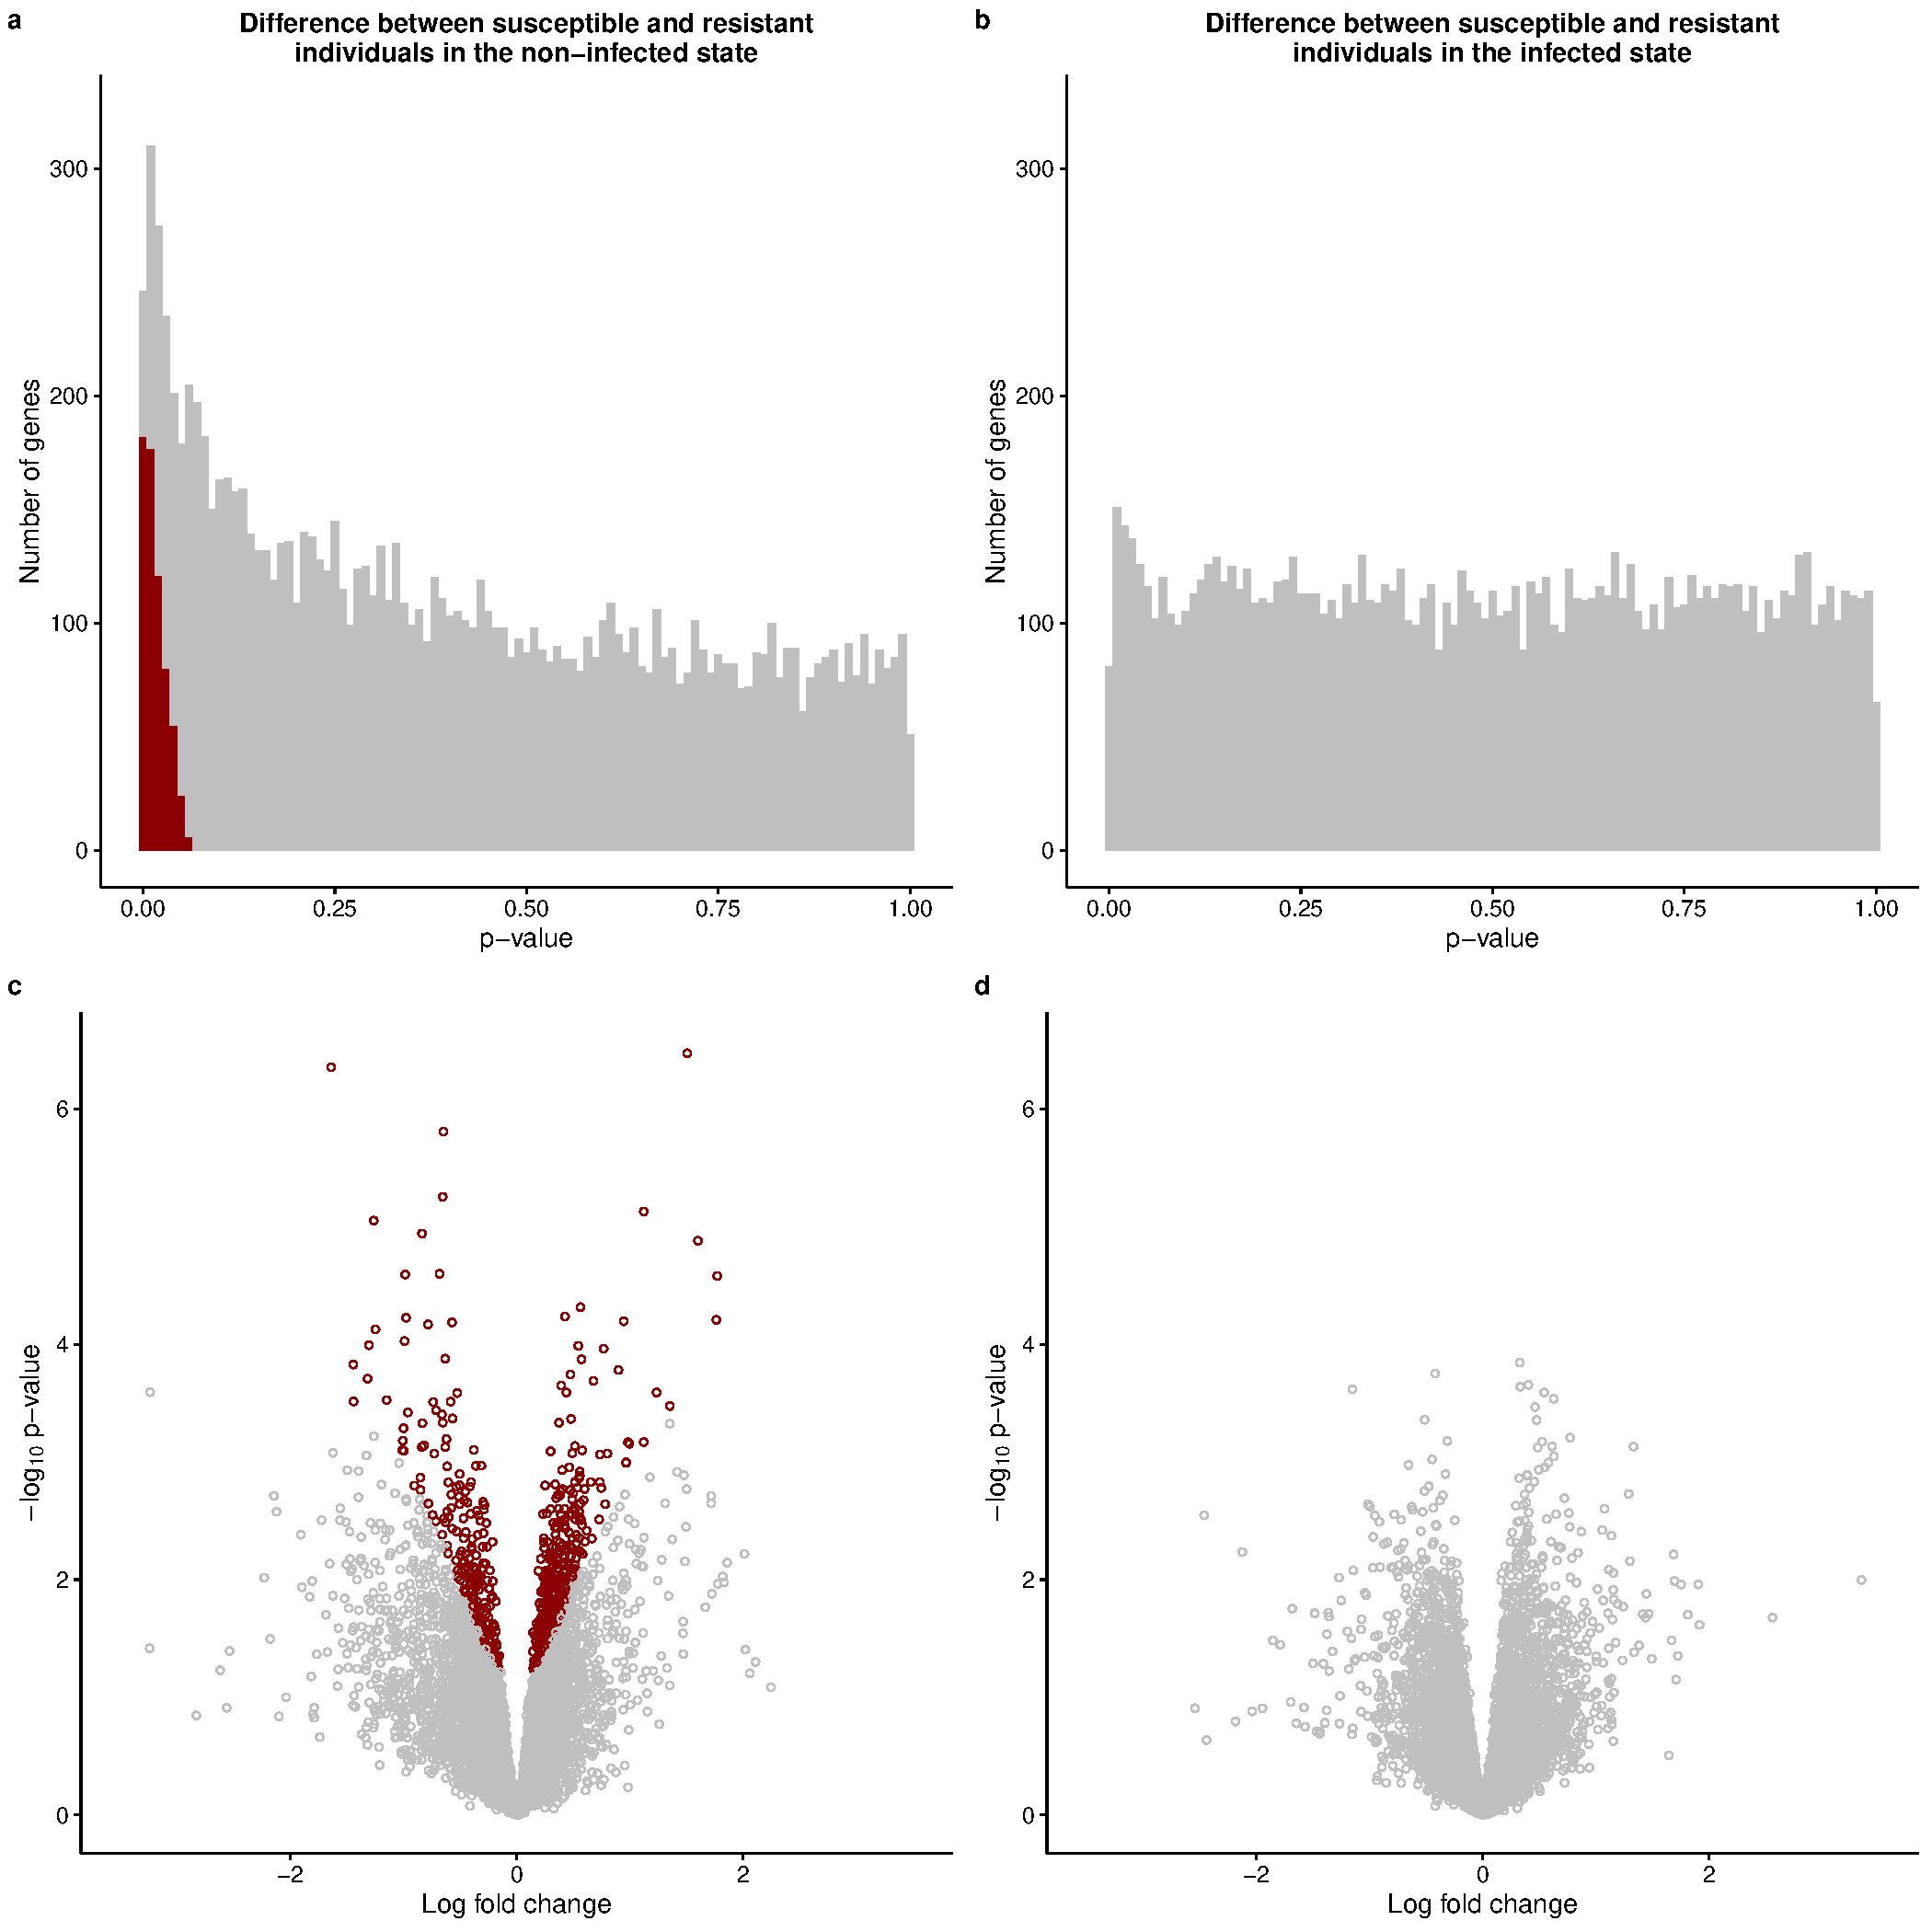
\includegraphics[width=5in]{img/ch03/limma.pdf}
\caption[Differential expression analysis.]{ \textbf{Differential
    expression analysis.} The top panel contains the distribution of
  unadjusted p-values after testing for differential expression
  between susceptible and resistant individuals in the (a)
  non-infected or (b) infected state. The bottom panel contains the
  corresponding volcano plots for the (c) non-infected and (d)
  infected states. The x-axis is the log fold change in gene
  expression level between susceptible and resistant individuals and
  the y-axis is the –log\textsubscript{10} p-value. Red indicates
  genes which are significant differentially expressed with a q-value
  less than 10\%.  }
\label{fig:limma}
\end{figure}

\subsection{iPSCs-based system effectively models primate endoderm differentiation}

Given the potential impact of study design properties on gene expression data and subsequent conclusions \cite{RN1402}, as a first step of our analysis, we confirmed that none of our recorded variables related to sample processing (apart from sample purity, as stated above) were confounded with our main variables of interest, namely day and species (see Methods; Additional file 1: Tables S4A-D; Additional file 2: Figures S2C and S5). Once we were confident that our study design provided an effective data set for addressing our biological questions of interest, we performed a global survey of the gene expression data using principal component analysis. This analysis indicated that the primary sources of gene expression variation are differentiation day (Figure 2A; Additional file 1: Tables S4A-E; regression of PC1 by differentiation day, P \textless 10-15), followed by species (regression of PC2 by species, P \textless 10-15). This observation was also supported by clustering analysis based on the correlation matrix of pairwise comparisons of the gene expression levels (Additional file 2: Figure S6).
After characterizing global gene expression patterns, we focused on the expression of specific transcription factors with known roles in developmental pathways (Figure 1C) and other previously known lineage specific markers \cite{RN1330, RN1328, RN1329}. Consistent with the results of our FACS analysis, we observed that the temporal trajectory of expression levels of known lineage specific markers and transcription factors further supported the assumed differentiation stages in each day (e.g. primitive steak-specific markers had increased expression on day 1, Figure 2B). The lineage specific markers and transcription factors were expressed at comparable levels in humans and chimpanzees at the relevant time points, consistent with previous literature \cite{RN1328, RN1329}, and further supporting the validity of our in vitro system (Additional file 2: Figure S7A).

\begin{figure}
\centering 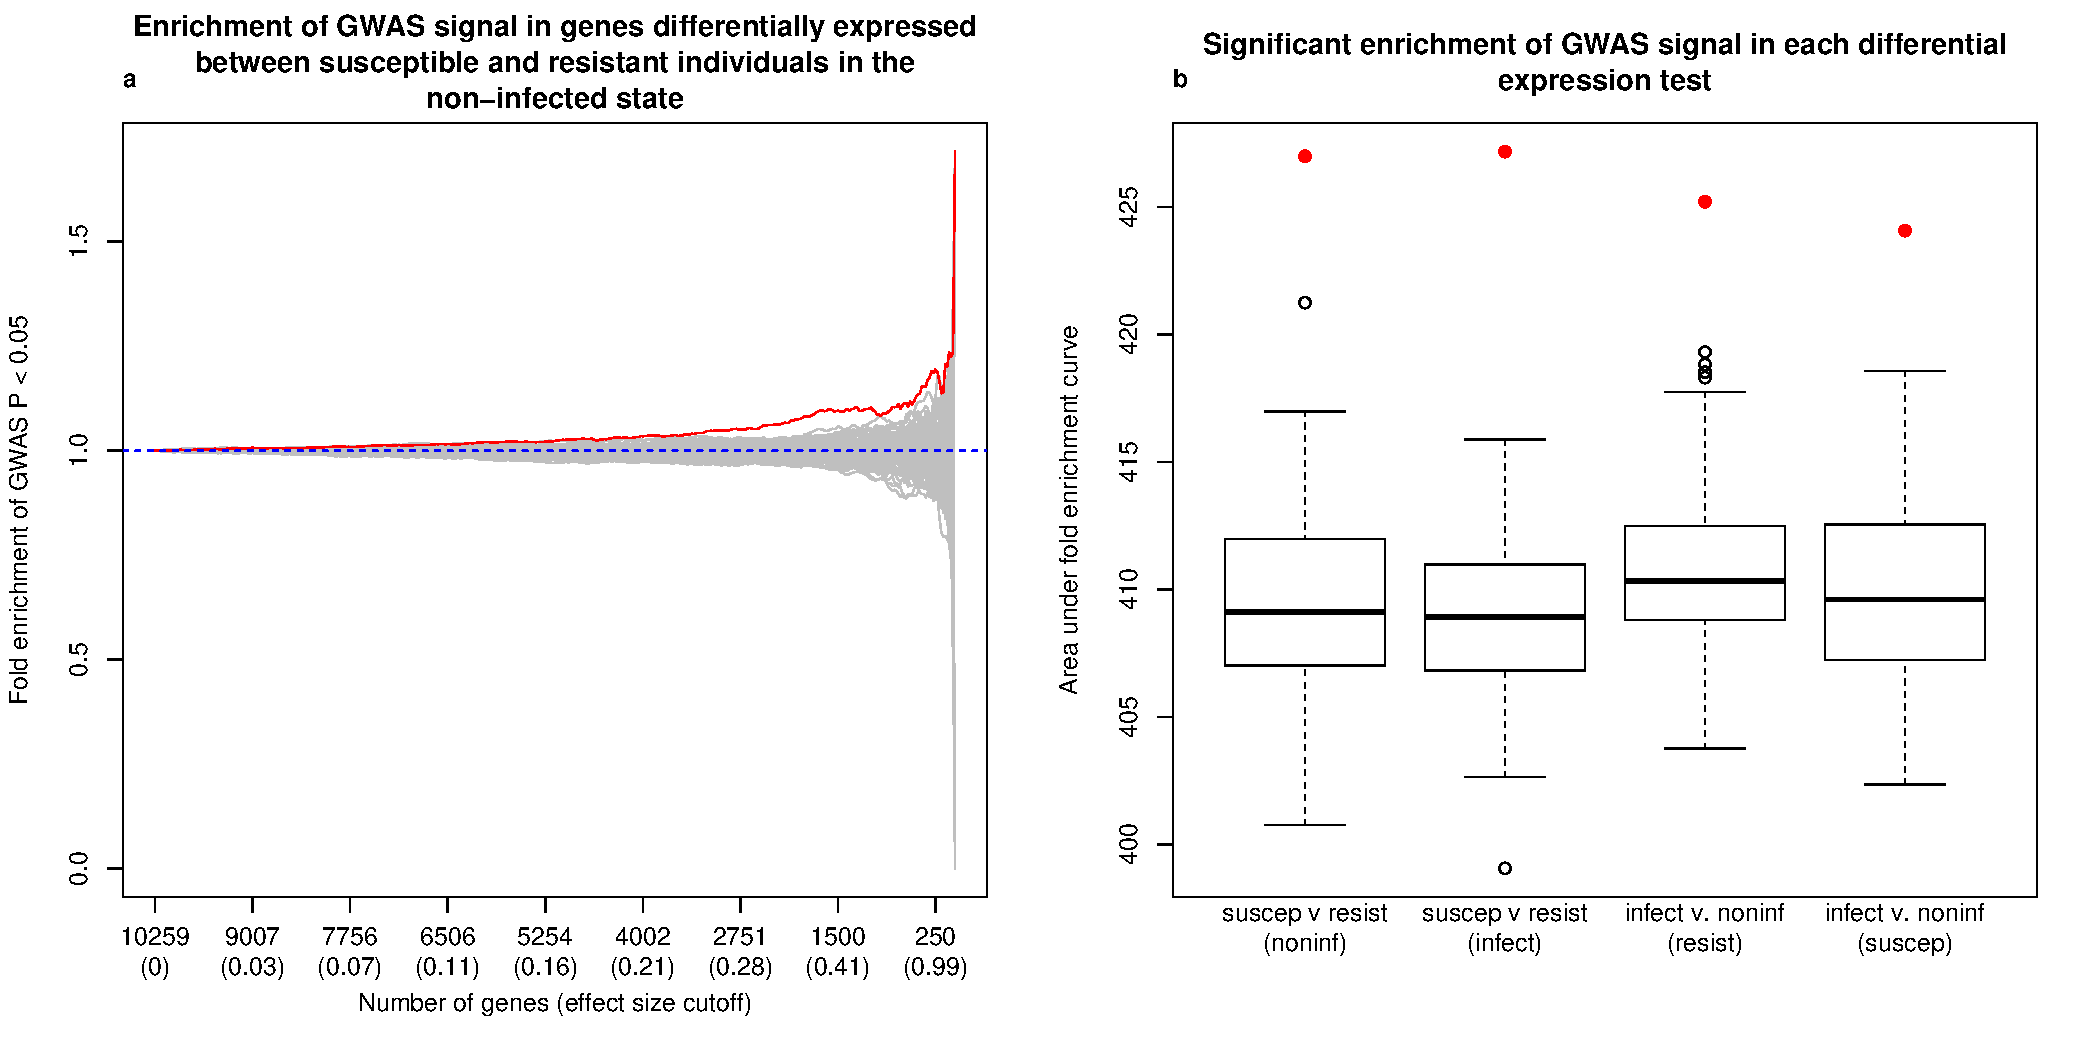
\includegraphics[width=5in]{img/ch03/gwas.pdf}
\caption[Comparison of differential expression and The Gambia GWAS
  results.]{ \textbf{Comparison of differential expression and The
    Gambia GWAS results.} (a) The y-axis is the fold enrichment
  (y-axis) of genes assigned a SNP with p-value less than 0.05 from
  the GWAS in The Gambia.The x-axis is bins of genes
  with increasingly stringent effect size cutoffs of the absolute log
  fold change between susceptible and resistant individuals in the
  non-infected state. The effect size cutoffs were chosen such that
  each bin from left to right contained approximately 25 fewer
  genes. The red line is the results from the actual data. The grey
  lines are the results from 100 permutations. The dashed blue line at
  y=1 is the null expectation. (b) The x-axis is each of the 4
  differential expression tests performed.  The y-axis is the area
  under the curve of the fold enrichment. The boxplot is the result of
  the 100 permutations, and the red point is the result from the
  actual data. As a reference, the leftmost boxplot corresponds to the
  enrichment plot in (a).  }
\label{fig:gwas}
\end{figure}

\subsection{Comparative assessment of gene expression changes during differentiation}

To identify gene expression differences between humans and chimpanzees throughout the timecourse, we used the framework of linear models (see Methods). We first assessed how many genes were differentially expressed (DE) between species at each time point independently. Using this approach, we classified thousands of genes as DE between the species (at FDR of 5\% 4475 ? 5077 genes are classified as inter-species DE at different times points; Figure 3A; Additional file 1: Tables S5A-D). Even at a fixed FDR cutoff, nearly half of the genes that were classified as DE between the species at any single time point were found to be DE in all time points (2269 genes). Nearly a third of genes whose expression was measured in our experiment were not classified as DE between the species at any time point (2862 genes, 28\%). 
We proceeded to consider temporal expression patterns within species. When analyzing expression changes across consecutive time points, we had more power to detect temporal gene expression differences in chimpanzee compared to humans (Figures 3B-C and 4; Additional file 1: Tables S6A-F), especially with respect to the transition between endoderm progenitors (day 2), and definitive endoderm samples (day 3). This property is likely related to the inter-species difference in purity of samples from these days, as discussed earlier. When we accounted for incomplete power (see ?Methods?), we found a remarkably consistent pattern whereby 77\% of DE genes between iPSCs and primitive streak in humans are also DE between these states in chimpanzees; similarly, 77\% of DE genes between primitive streak and endoderm progenitors in humans are also DE between these states in chimpanzees; and 80\% of DE genes between endoderm progenitors and definitive endoderm in humans are also DE between these states in chimpanzees (Additional file 1: Table S7). As might be expected from these observations, we found that the relationship between day and gene expression was largely independent of species (Figure 3D; Additional file 1: Table S8A-C).

\begin{figure}
\centering 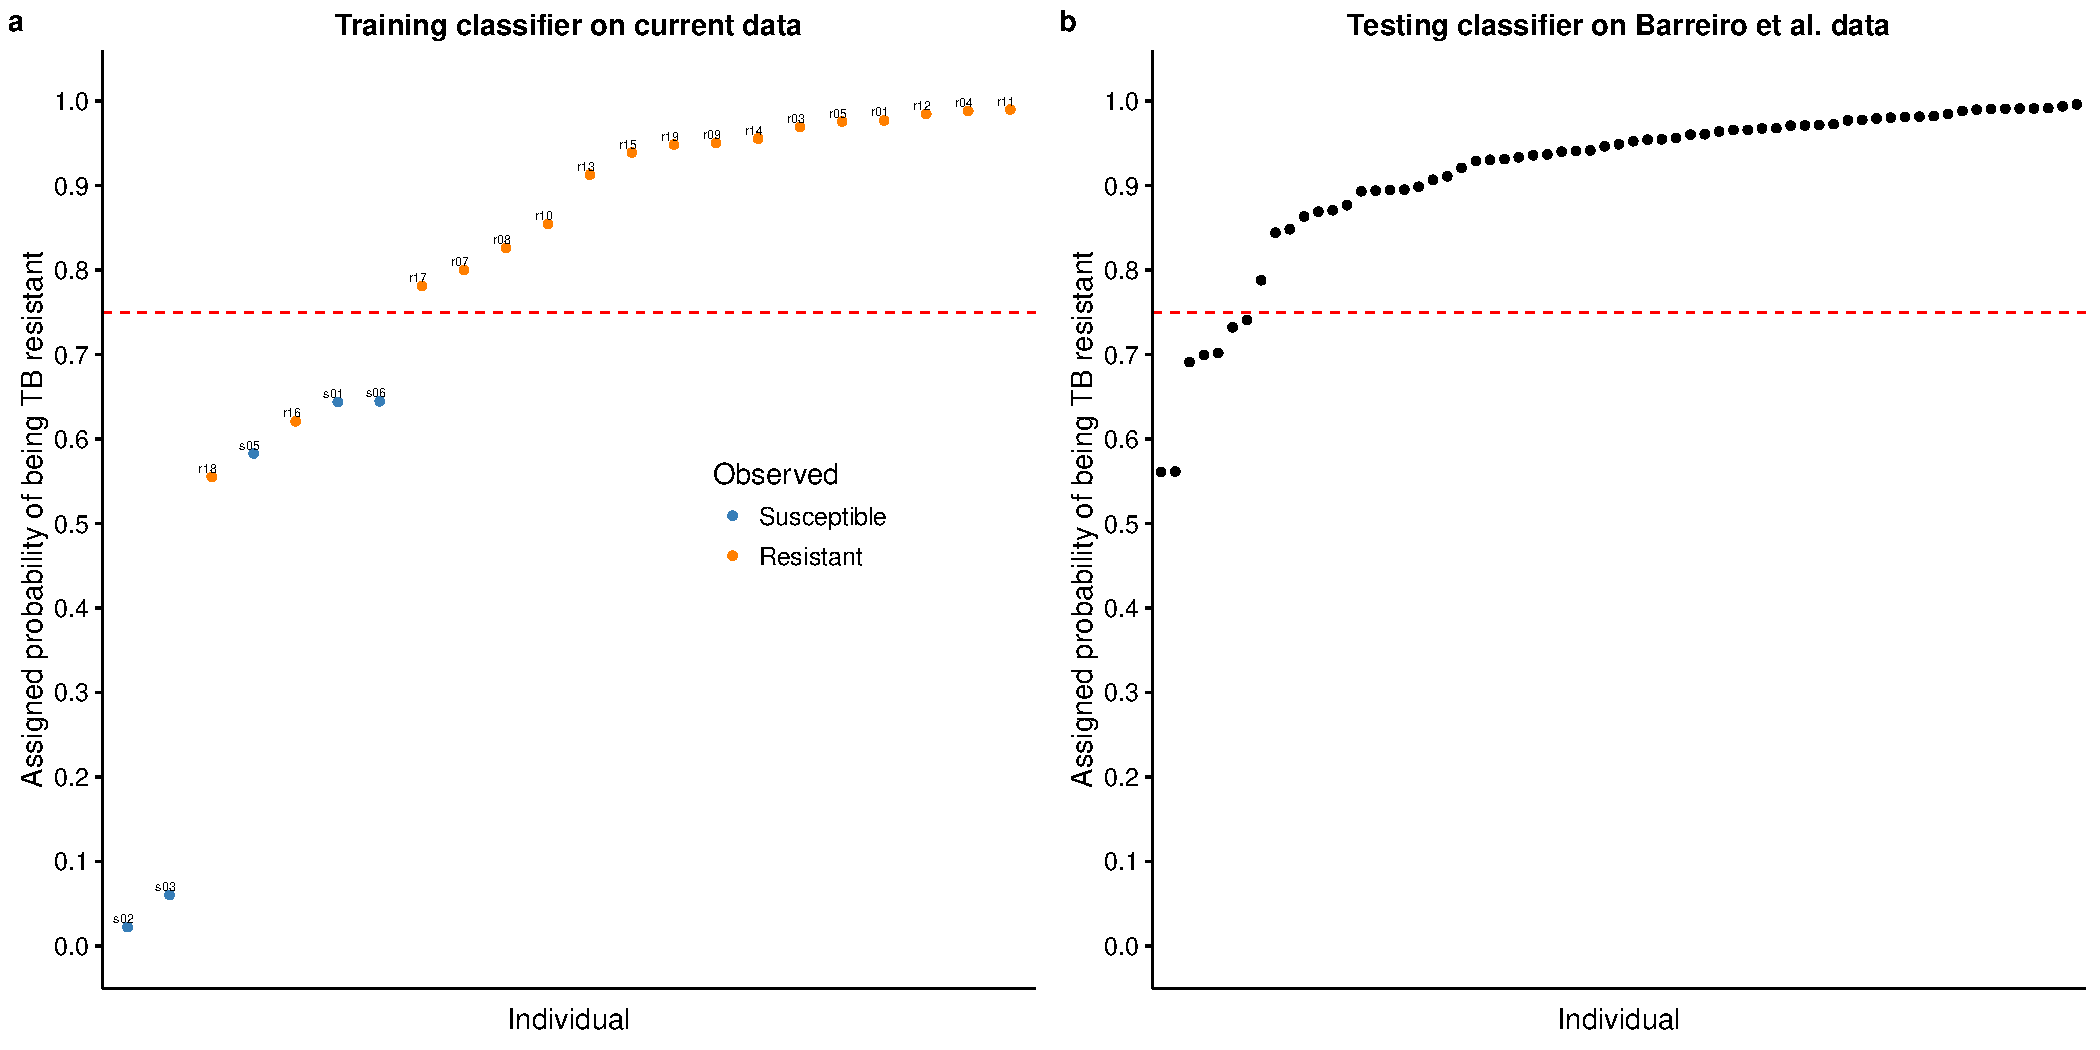
\includegraphics[width=5in]{img/ch03/classifier-svm.pdf}
\caption[Classifying TB susceptible individuals using a support vector
  machine model.]{ \textbf{Classifying TB susceptible individuals
    using a support vector machine model.} (a) The estimates of
  predicted probability of TB resistance from the
  leave-one-out-cross-validation for individuals in the current
  study. The blue circles represent individuals known to be
  susceptible to TB, and orange those resistant to TB. The horizontal
  dashed red line at a probability of 0.75 separates susceptible and
  resistant individuals. (b) The estimates of predicted probability of
  TB resistance from applying the classifier trained on the data from
  the current study to a test set of independently collected healthy
  individuals.  }
\label{fig:classifier}
\end{figure}

\subsection{Joint Bayesian analysis reveals conservation of temporal gene expression profiles}

In an attempt to further overcome issues of incomplete power affecting these original na�ve pairwise DE comparisons, and to account for dependency in data from different time points, we utilized a Bayesian clustering approach implemented by Cormotif \cite{RN1908}. This joint modeling technique leverages expression information shared across time points to identify the most common temporal expression patterns (referred to as ?correlation motifs?). 
We identified diverse expression patterns that emerge as differentiation progresses in both species (Figure 5; Additional file 1: Table S9A) as well as a set of 3789 genes whose expression is not significantly altered throughout the timecourse (8004 genes could be reliably classified into a motif, Additional file 1: Table S9A; Additional file 2: Figure S8A). This analysis revealed further evidence for conserved gene expression patterns, as 75\% of genes assigned were assigned to motifs with the same or similar temporal regulatory trajectories in both species (Figure 5). Further, when we excluded data from the definitive endoderm samples, where we suspect that a particularly large inter-species difference in sample purity has increased gene expression variance between the species, we assigned 85\% of genes to motifs with the same temporal trajectories across species. These observations are robust with respect to the number of correlation motifs, the method used to combine data from technical replicates, which days were included in the pairwise comparisons, and the inclusion of all 10,304 genes in the analysis (Additional file 2: Figures S8B-D and S9; Additional file 4). Our observations are also robust with respect to the overall approach used to estimate and compare gene expression trajectories (Additional file 2: Figure S7B; Additional file 4).
We found two correlation motifs with a potential marked difference between the species at a given stage (motif 4 with 187 genes and motif 7 with 686 genes). In both of these motifs, data from the earliest time points were conserved but gene regulation in the final stage (day 2 to 3) differed between the species. The genes in these motifs were enriched for Gene Ontology (GO) annotations related to animal organ development (e.g. \textit{NRTN, PITX2, RDH10}), anatomical structure morphogenesis (\textit{ARHGDIA, EHD2, SERPINE1}), regulation of developmental process (\textit{FLRT3, LOXL2, SEMA7A}), and regulation of cell differentiation (\textit{DIXDC1, ENC1, IRF1}; Additional file 1: Table S9B) \cite{RN1783}. These four GO annotations were not enriched in other similarly sized motifs or group of motifs (Additional file 1: Tables S9C-E) \cite{RN1783, RN1794}. Unfortunately, due to interspecies differences in purity at the later days, we cannot definitively determine whether these enrichments are driven by biological or technical differences. 

\subsection{Reduced variation in gene expression levels at primitive streak}

We next turned our attention to differences in the magnitude of variation in gene expression levels across time points, within and between species. Previous studies reported that variation in gene expression levels between individuals was lower in iPSCs than in differentiated cells (\cite{RN1399, RN2196} and Additional file 2: Figure S10A). We were thus interested in gene expression variation during iPSC differentiation in our comparative system. 
We first compared within-species expression variation for all 10,304 orthologous genes across time points. We found a reduction in inter-individual variation of gene expression levels as the human samples differentiated from iPSCs to primitive streak (P \textless 10-15, Figure 6). We also detected this pattern when we considered the chimpanzee samples (P \textless 10-15, Figure 6), but the effect size in chimpanzee is much smaller. We did not identify similar reduction in variation in gene expression levels in any other transition during the timecourse in either species (P \textgreater 0.5 for testing the null of no change in variance of gene expression from day 1 to 2 and from day 2 to 3 in each species). As mentioned above, the purity of the samples in days 2 and 3 is lower than that of samples in days 0 and 1, though we only successfully measured the purity values for the samples that were processed in the second batch. We accounted for the measured purity values by regressing them out of the gene expression data. As might be expected, accounting for the purity values resulted in different patterns observed for the data from days 2-3. Yet, the reduction in variation from day 0 to 1 persisted in both species even after we accounted to the purity values (Additional file 2: Figure S10B).
We turned our attention to regulatory divergence between species. The overall human-chimpanzee divergence in gene expression levels was also slightly reduced as samples differentiated from iPSCs to primitive streak (Mann-Whitney U Test, P = 0.04; Additional file 2: Figure S10C), but not in any other transition during the timecourse. Furthermore, while we classified 504 genes as DE between humans and chimpanzees exclusively in iPSCs (of a total of 4,475 DE genes in iPSCs, FDR = 5\%; Figure 3A; Additional file 1: Table S10), we found only 279 genes that were DE exclusively in primitive streak samples (from a total of 4,408 DE genes for the primitive streak; Figure 3A; Additional file 1: Table S10). The number of genes that are DE between the species exclusively in endoderm progenitors and definitive endoderm samples is higher (at FDR of 5\%, 402 and 934, respectively; Figure 3A; Additional file 1: Table S10). The observation of a smaller number of genes that are DE exclusively in primitive streak samples compared with iPSCs is robust with respect to normalization method, purity of the samples, FDR cutoff, and differentiation batch (Additional file 1: Table S10; Additional file 2: Figures S2C, 10C and S11). While the difference in divergence and the number of DE genes between these differentiated states is modest, and could potentially be explained by a number of non-biological factors (including the differences in purity in the later day), this observation was intriguing to us.
We thus focused on the transition between iPSCs to primitive streak in both species. The recorded technical factors (including purity for these states) are highly similar across biological conditions in days 0 and 1, and therefore are not likely to explain this observation (Additional file 1: Table S11). We thus proceeded to analyze the trajectory of variation in expression level on an individual gene basis. In this analysis, we were particularly interested to address whether the individual genes that undergo a change in variation of expression levels are shared across species. An observation of excess sharing could not be explained by inter-species differences in technical factors and hence would provide substantial support to the notion of conserved reduction of regulatory variation as the samples begin their differentiation process.
We used F tests to identify genes whose within-species variation in expression levels differs across time points (see ?Methods?). Distributions of P values from all tests can be found in Figures 7A-B and Additional file 1: Tables S12A-B, which indicate that for a large number of genes, within-species variation in expression levels were reduced exclusively in primitive streak samples. Indeed, while we did not have much power to detect differences in variation of individual gene expression levels between states (due to the small number of individuals in each species), we observed a clear excess of small P values when we tested the null hypothesis that there was no reduction in gene expression levels from day 0 to 1. Using Storey?s approach \cite{RN1393} to account for incomplete power, we estimated that within-species variation in expression levels was reduced as the samples differentiate from iPSCs to primitive streak in 83\% and 27\% of human and chimpanzee genes, respectively (Figures 7A-B). This result was robust with respect to the method used to calculate the proportion of true positives \cite{RN1392} (Additional file 2: Figure S12). We did not observe reduced variation of gene expression in any other differentiation state in our data (Figures 7; Additional file 2: S13A).
We next asked about the overlap of genes with reduced variation in primitive streak samples across the two species. Specifically, we asked whether human genes with lower within-species variation in expression levels in primitive streak are more likely to show the same pattern in chimpanzee genes. For this analysis, we again used the Storey approach \cite{RN1393} to estimate the proportion of true positive tests in one species, conditional on the observation of reduced variation in the other species (see Methods). We estimated that 47\% of genes whose variation in expression level is reduced in human primitive streak samples showed a similar pattern in chimpanzees (under a permuted null we expect 27\%, P \textless 10-4, Figure 7C; Additional file 1: Table S13). When we condition on observing a reduction of variation in chimpanzees, the overlap with humans was 84\% (under a permuted null we expect 83\%, P = 0.38; Figure 7D). This high value was not unexpected because of the initial large proportion of human genes with a clear signature of reduced variation in primitive streak. Because any technical differences that are confounded with species would contribute to increased inter-species differences, these observations support, yet probably underestimate, the degree of high conservation of regulatory patterns in humans and chimpanzees. 
Using a similar approach to account for incomplete power, we also found a marked overlap of genes whose expression underwent a significant increase in variation throughout the transition from primitive streak to endoderm progenitors (Figures 7E-F; Additional file 2: Figure S13B). All our observations were robust to a wide range of statistical cutoffs used to classify genes whose within-species variation changes across the differentiation states (Additional file 2: Figures S14-S16). In particular, because these are reports of conserved patterns, they are likely to underestimate the degree of conservation given technical differences between the species, including the difference in purity of the samples in days 2 and 3.
Finally, we sought to provide insight into the potential functional consequences of our observations. Interestingly, genes that show reduction of variation in gene expression levels in both species are enriched for GO annotations \cite{RN1783} related to development, including neuroepithelial cell differentiation (e.g. \textit{MYCL, NODAL, CDH2}), cell migration during gastrulation (\textit{FGF8, MIXL1}), and trophectodermal cell differentiation (\textit{CNOT3, EOMES, SP3}; Additional file 1: Table S14). Moreover, we found that null mutation in mouse orthologs \cite{RN2197} of the primate genes with shared reduction of expression variation in our study were more highly associated with embryonic lethality than null mutation in mouse orthologs of primate genes that did not show that pattern (41\% versus 28\%, P \textless 10-4 \cite{RN2198, RN1797}). 


\section{Discussion}

Our results indicate a strongly conserved temporal expression profile across species during early differentiation. We observed a large number of genes with similar expression profiles across species. Indeed, we found that DE genes between differentiation states are shared between the two species far beyond what expected by chance alone. When we jointly analyzed data from the entire timecourse, nearly all the gene expression trajectory motifs we identified, including 75\% of all genes assigned to a motif, are shared across the two species (Figure 5). Still, our observations likely underestimated the proportion of shared regulatory patterns due to incomplete power.
Our finding that regulatory trajectories throughout endoderm differentiation are generally highly conserved in these two species was expected. Yet, our observation that a large number of genes are associated with conserved reduced regulatory variation in a specific transition state is a somewhat surprising property. Indeed, in our opinion, the most significant finding of this study is the observation that regulatory variation is reduced in both humans and chimpanzees as the cell cultures differentiate from iPSCs to primitive streak. We found a marked overlap between the species in the specific genes that experience this reduction of regulatory variance, indicating high degree of conservation in this process.
Before we discuss the potential implications of our observations, we will first discuss a few considerations regarding the iPSC based differentiation models. We argue that the use of iPSC models allows for greater control and transparency of comparative studies in primates, including a better appreciation of caveats that have always affected such studies but were typically cryptic. 
For more than a decade, comparative genomics in primates has relied on the use of frozen tissues. An implicit assumption underlying the use of these tissues has been that they faithfully reflect interspecies gene regulatory similarities and differences. Yet, we know that gene regulation in these tissues was likely impacted by non-genetic factors, such as the individual?s diet, age, and cause of death. In addition, it is nearly impossible to stage frozen tissues with respect to cellular composition. In fact, in practically all studies of comparative data from frozen tissues, cellular composition was not even measured. Indeed, comparative studies of gene expression in primate frozen tissue samples, including those by our own group, simply assumed that most observed patterns are driven by genetic control. 
In contrast to frozen tissues, the primate iPSC-based differentiation model allows us to minimize the impact of non-genetic (e.g. environmental) factors. We can also control to a large extent the cellular composition of the samples, and more importantly, we can measure and account for differences in cellular composition. Comparative experiments with iPSC-based differentiation are certainly not flawless, but they allow us to more explicitly characterize, and often account for, confounding factors than it was possible with frozen tissue samples. In the case of the current study, we used human and chimpanzee iPSC lines that were generated, and differentiated, using the same protocols. We made considerable efforts to balance the majority of sample processing properties related to our study design with respect to species and time point. For example, the two differentiation batches we used included multiple human and chimpanzee lines (which we also balanced with respect to gender). Admittedly, in vitro differentiation protocols are not identical to natural developmental signaling and natural cell-driven developmental processes may be overridden by our administered media conditions. Moreover, although we used an identical differentiation protocol across the entire experiment, we observed a wide distribution of cell purity across samples, with a marked difference between the species in the purity of cultures form days 2 and 3. 
 The fact that we are able to measure and discuss purity and cellular composition as a potential flaw in our study is an advantageous property of the iPSC-based differentiation system. At present, we cannot exclude the possibility that the observed differences in cellular heterogeneity across time points may have driven the observation of reduced regulatory variation exclusively in primitive streak samples. In our opinion, however, this is unlikely, though our arguments are mostly circumstantial and we will not be able to provide a definitive answer without additional single cell experiments (which will be the scope of a future study). Our intuition is based on the following properties: First, the iPSC cultures are the most homogenous in our experiment and we nevertheless observe a reduction of variation in gene expression levels in day 1 samples. Second, the conclusion of high sharing and similarities between species should be robust (conservative, in fact) with respect to technical differences between species, including in purity. Third, when we account for the purity values measured for the second batch of samples, the relative expression patterns remain similar.
That said, to provide definitive answer, we will revisit these questions with an experimental design that involves single cell data from the same comparative differentiation trajectory. Single cell RNA sequencing data will also be able to shed light on our observation that gene regulation in definitive endoderm (day 3), unlike earlier days, does not indicate strong conservation between the species. In definitive endoderm samples, we observed the largest number of DE genes across species, the smallest number of DE genes between two consecutive time points in humans, and the lowest overlap in DE genes between time points. Unlike in the human samples, the chimpanzees had a relatively consistent number of DE genes between any two consecutive time points. Some of these observations might be explained by the cell purity difference between species. 
It should be noted that the effect sizes for the reduction in variation from day 0 to 1 are small in the chimpanzee samples and that the P value distributions do appear quite different across species. These differences, however, do not invalidate our finding that there is a significant overlap of genes that undergo a reduction of variation in gene expression levels in both species. If the reduction of variation in gene expression levels were spurious within each species, then we would not expect a statistically significant overlap of such genes. The observation of reduced regulatory variation is rather unusual in general, partly due to the unusual design of our study. Indeed, only few comparative studies have been designed to allow one to measure changes in variation over time. One such example, from a completely different context, can be found in a previous study in which monocytes from humans, chimpanzees, and rhesus macaques, which were stimulated with lipopolysaccharide (LPS) to mimic infection \cite{RN1400}. When comparing gene expression in LPS-stimulated monocytes to that of non-stimulated cells, the authors found a reduction of inter-species variation in gene expression levels in a number of key transcription factors involved in the regulation of TLR4-dependent pathways. 
In our study, we found enrichment for genes in developmental pathways among genes with conserved reduction of expression variation. This observation is consistent with the notion \cite{RN1386} that developmental pathways need to be tightly regulated in general. This notion is also supported by deep conservation and lethality upon disruption seen in many of these genes. Null mutations in mouse orthologs of over 40\% of the genes with conserved reduced regulatory variation at primitive streak are associated with embryonic lethality. For example, \textit{Xenopus laevis} embryos with null mutations in the ortholog of human \textit{MIXL1} exhibit abnormalities in primitive streak and node formation \cite{RN1553}. Similarly, homozygous null \textit{MIXL1} mice have abnormal mesoendoderm development and do not survive to birth \cite{RN1646}. \textit{EOMES} homozygous null mice lack trophoectoderm outgrowth \cite{RN1760} and do not properly form the definitive endoderm \cite{RN1772}. This mutation is lethal early in gestation. Overall, regulation of these genes is likely to be finely tuned at early development. 
 Indeed, reduced regulatory variation early in the endoderm differentiation process may be driven by the property of canalization during development. The theory of canalization posits that developmental processes end in a finite number of states despite minor environmental perturbations \cite{RN1391, 1386, 1387}. Canalization is fundamentally linked to evolutionary states \cite{RN1387}, and thus phenotypic robustness; therefore, even when reduced variation in gene expression levels is observed in cell culture, the explanation of canalization is intuitively appealing considering the discrete nature of cell types in an adult animal. Our results suggest that stages subsequent to primitive streak may follow a more relaxed transcriptional regulation with higher influence of individual genotypes. 
Our observations may be consistent with activation of deeply conserved regulatory programs at the initial stages of gastrulation followed by processes less affected by evolutionary constraint and therefore potentially more amenable to adaptation. In other words, our results supports the expectation that gastrulation is a highly canalized and conserved process in humans and chimpanzees.�More generally, we believe that despite limitations to studying comparative development using iPSC models, which we have discussed, this system provides the opportunity to study previously unappreciated aspects of primate biology.�

\section{Methods}

\subsection{Ethics Statement}

\subsection{Data availability}


\section{Acknowledgments}

We thank T. Thye for sharing the GWAS data with us. This study was
funded by National Institutes of Health (NIH) Grant AI087658 to YG and
LT. JDB was supported by NIH T32GM007197. The content is solely the
responsibility of the authors and does not necessarily represent the
official views of the NIH.

%\clearpage\newpage
\section{Supplementary Information}\label{ch03-supplementary-information}

\subsection{Supplementary Figures}

\begin{figure}[!htb]
\centering 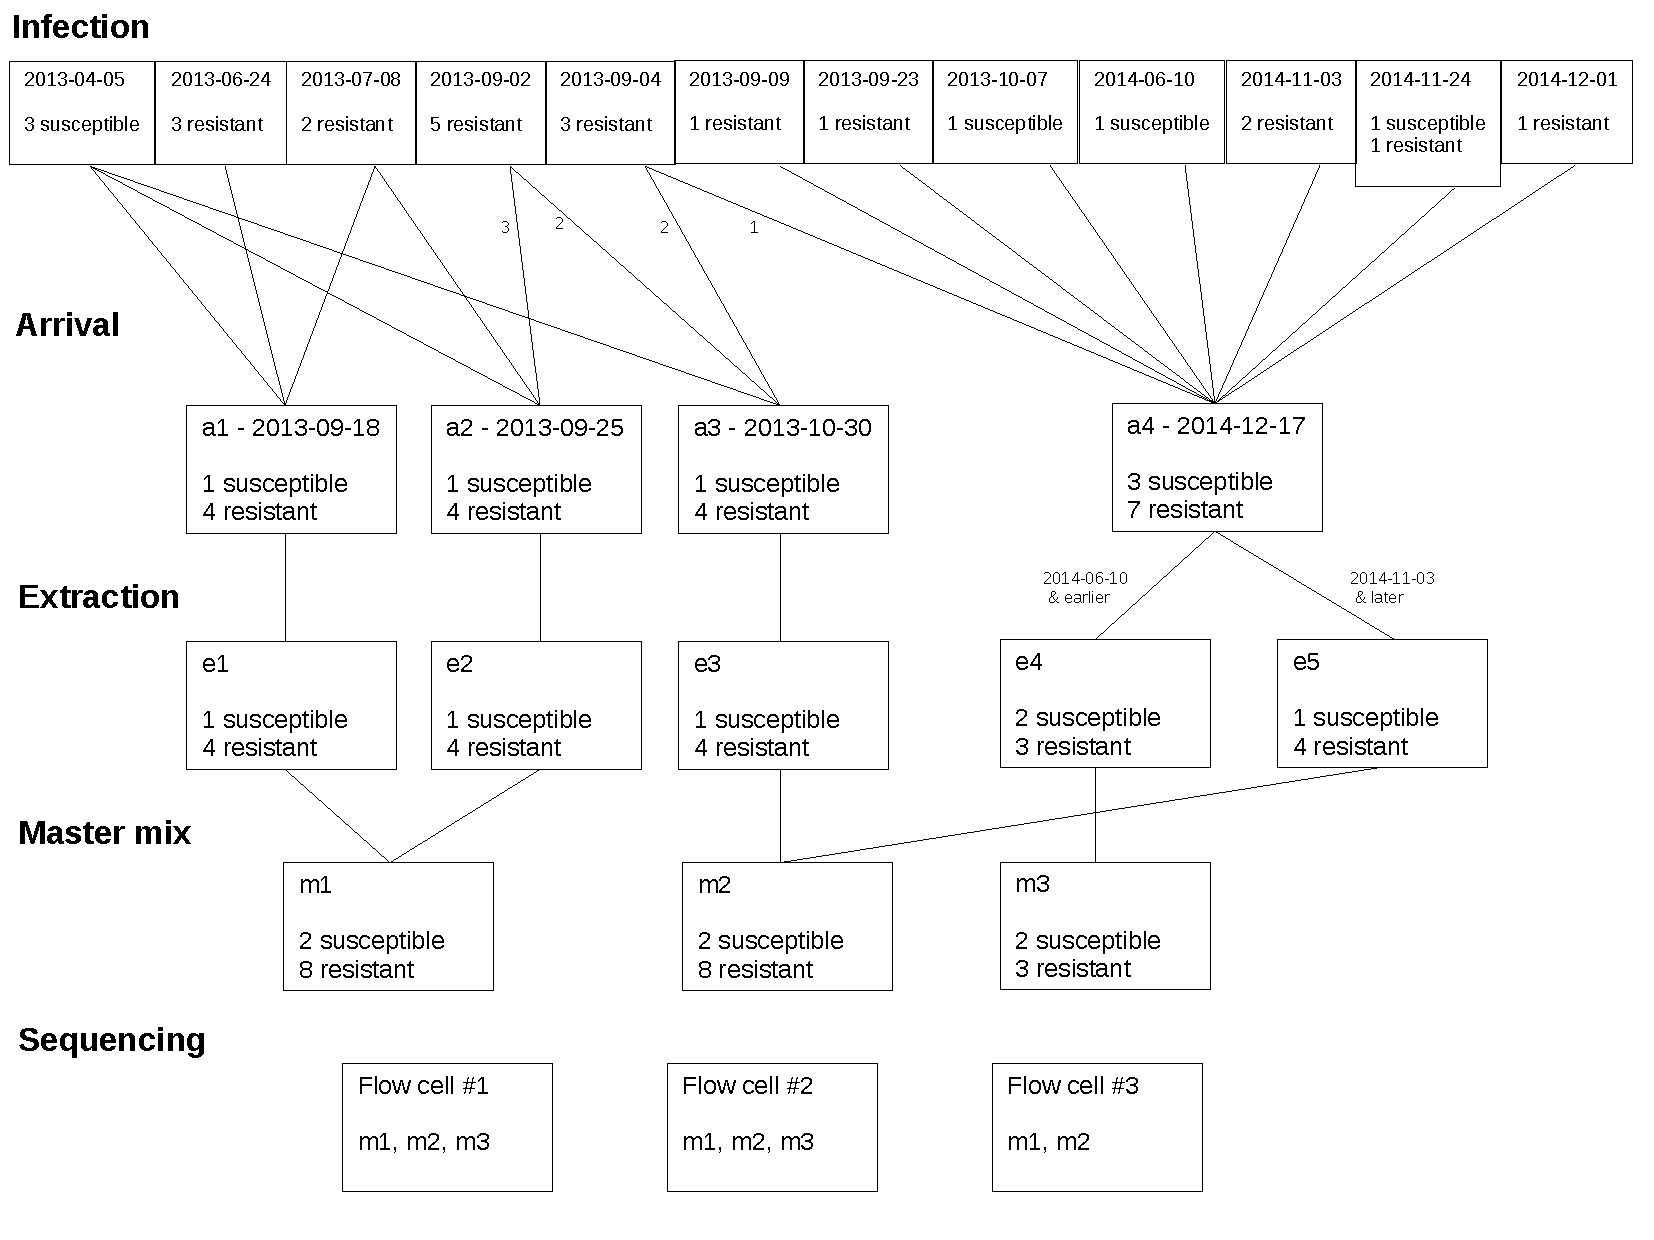
\includegraphics[width=5in]{img/ch03/processing.pdf}
\caption[Batch processing.]{ \textbf{Batch processing.} We designed
  the processing of the samples to minimize the introduction of
  technical batch effects. Specifically, we attempted to balance the
  processing of samples obtained from susceptible and resistant
  individuals. In the diagram, each box represents a
  batch. ``Infection'' labels the batches of the infection
  experiments, ``Arrival'' labels the batch shipments of cell lysates
  arrived in Chicago, USA from Paris, France, ``Extraction'' labels
  the batches of RNA extraction, ``Master Mix'' labels the batches of
  library preparation, and ``Sequencing'' labels the batches of flow
  cells. Each master mix listed in a flow cell batch was sequenced on
  only one lane of that flow cell.  }
\label{fig:process}
\end{figure}


\begin{figure}[!htb]
\centering
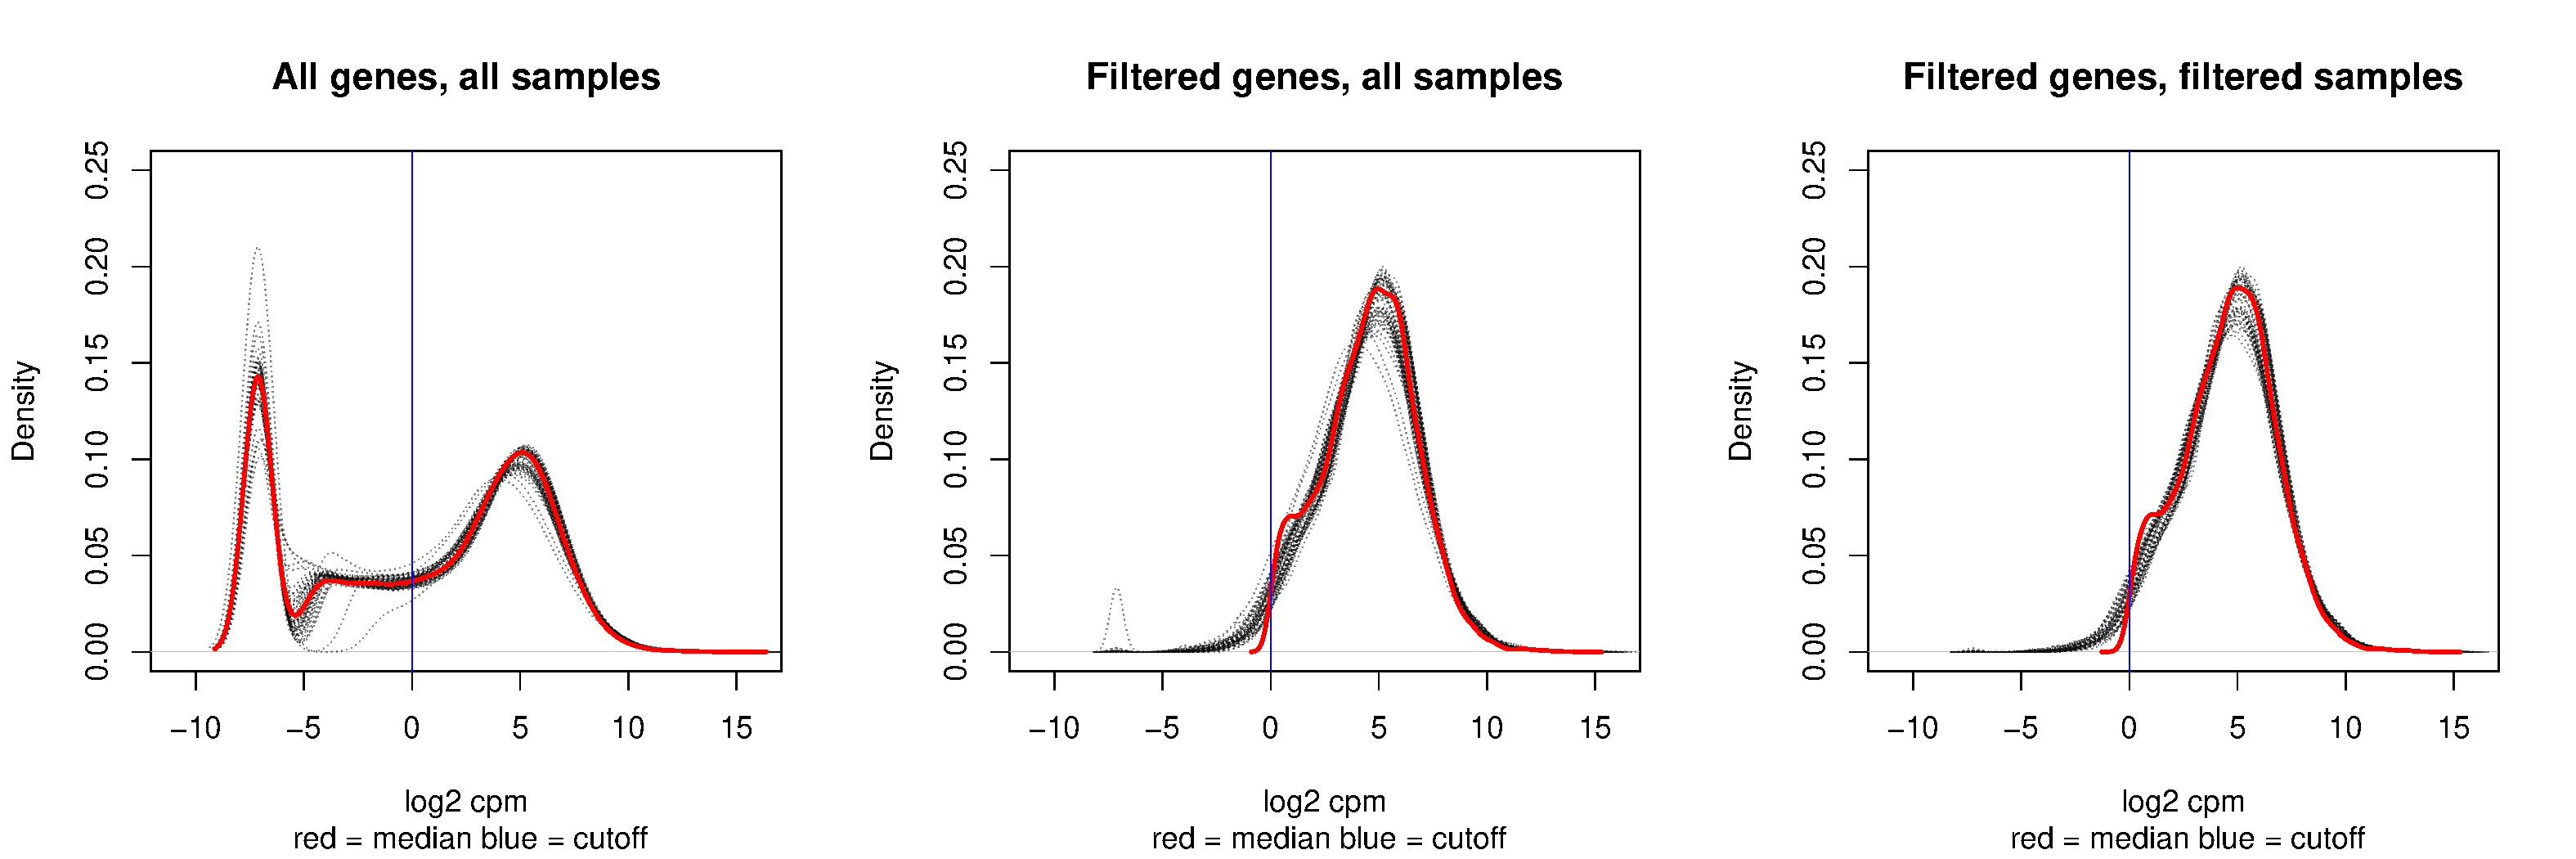
\includegraphics[width=5in]{img/ch03/gene-exp-distribution.pdf}
\caption[Gene expression distributions before and after filtering
  genes and samples.]{ \textbf{Gene expression distributions before
    and after filtering genes and samples.} The log\textsubscript{2}
  counts per million (cpm) of each sample is plotted as a dashed gray
  line. The solid red line represents the median value across all the
  samples. The vertical solid blue line at $x = 0$ represents the
  cutoff used to filter lowly expressed genes based on their median
  log\textsubscript{2} cpm. The left panel is the data from all 19,800
  genes and 50 samples, the middle panel is the data from the 11,336
  genes remaining after removing lowly expressed genes, and the right
  panel is the data from 11,336 genes and the 44 samples remaining
  after removing outliers.  }
\label{fig:gene}
\end{figure}

\begin{figure}[!htb]
\centering
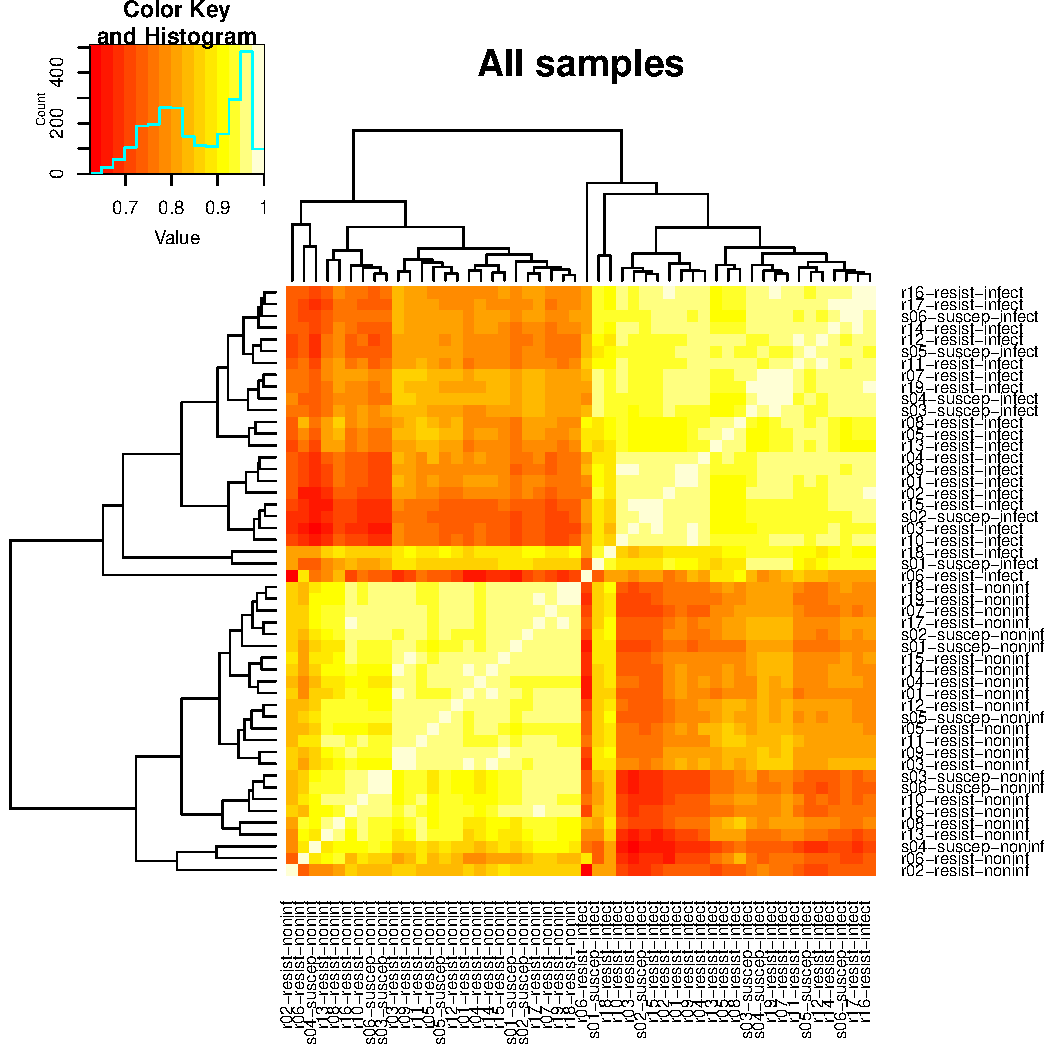
\includegraphics[width=5in]{img/ch03/heatmap-all-samples.pdf}
\caption[Heatmap of correlation matrix of samples.]{ \textbf{Heatmap
    of correlation matrix of samples.} Each square represents the
  Pearson correlation between the log\textsubscript{2} cpm expression
  values of two samples. Red indicates a low correlation of zero and
  white represents a high correlation of 1. The dendrogram displays
  the results of hierarchical clustering with the complete linkage
  method.  The outliers of the non-infected samples are
  s04-suscept-noninf, r02-resist-noninf, and r06-resist-noninf. The
  outliers of the infected samples are s01-suscep-infect,
  r06-resist-infect, and r18-resist-infect.  }
\label{fig:heat-all}
\end{figure}

\begin{figure}[!htb]
\centering
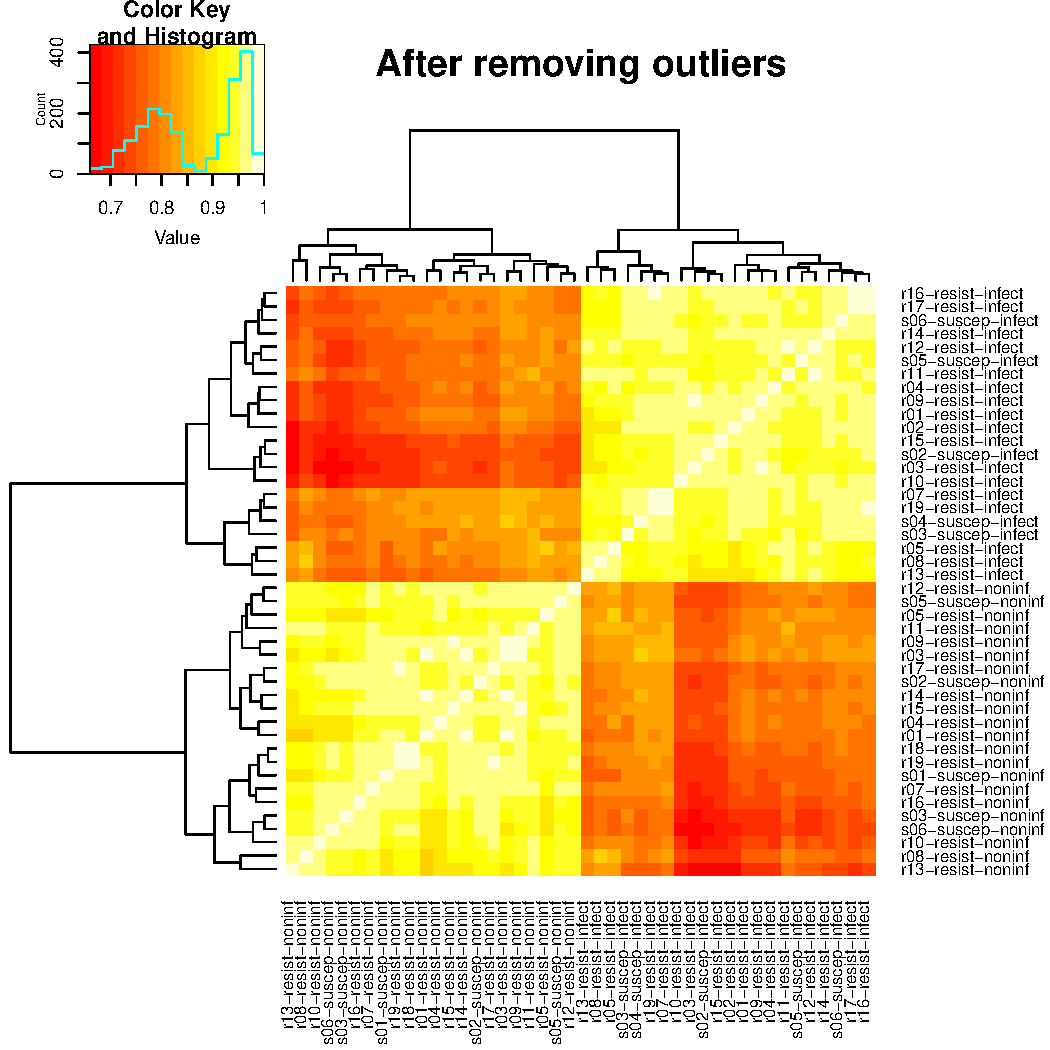
\includegraphics[width=5in]{img/ch03/heatmap-no-outliers.pdf}
\caption[Heatmap of correlation matrix after removing outliers.]{
  \textbf{Heatmap of correlation matrix after removing outliers.} Each
  square represents the Pearson correlation between the
  log\textsubscript{2} cpm expression values of two samples. Red
  indicates a low correlation of zero and white represents a high
  correlation of 1. The dendrogram displays the results of
  hierarchical clustering with the complete linkage method.  }
\label{fig:heat-filt}
\end{figure}


\begin{figure}[!htb]
\centering 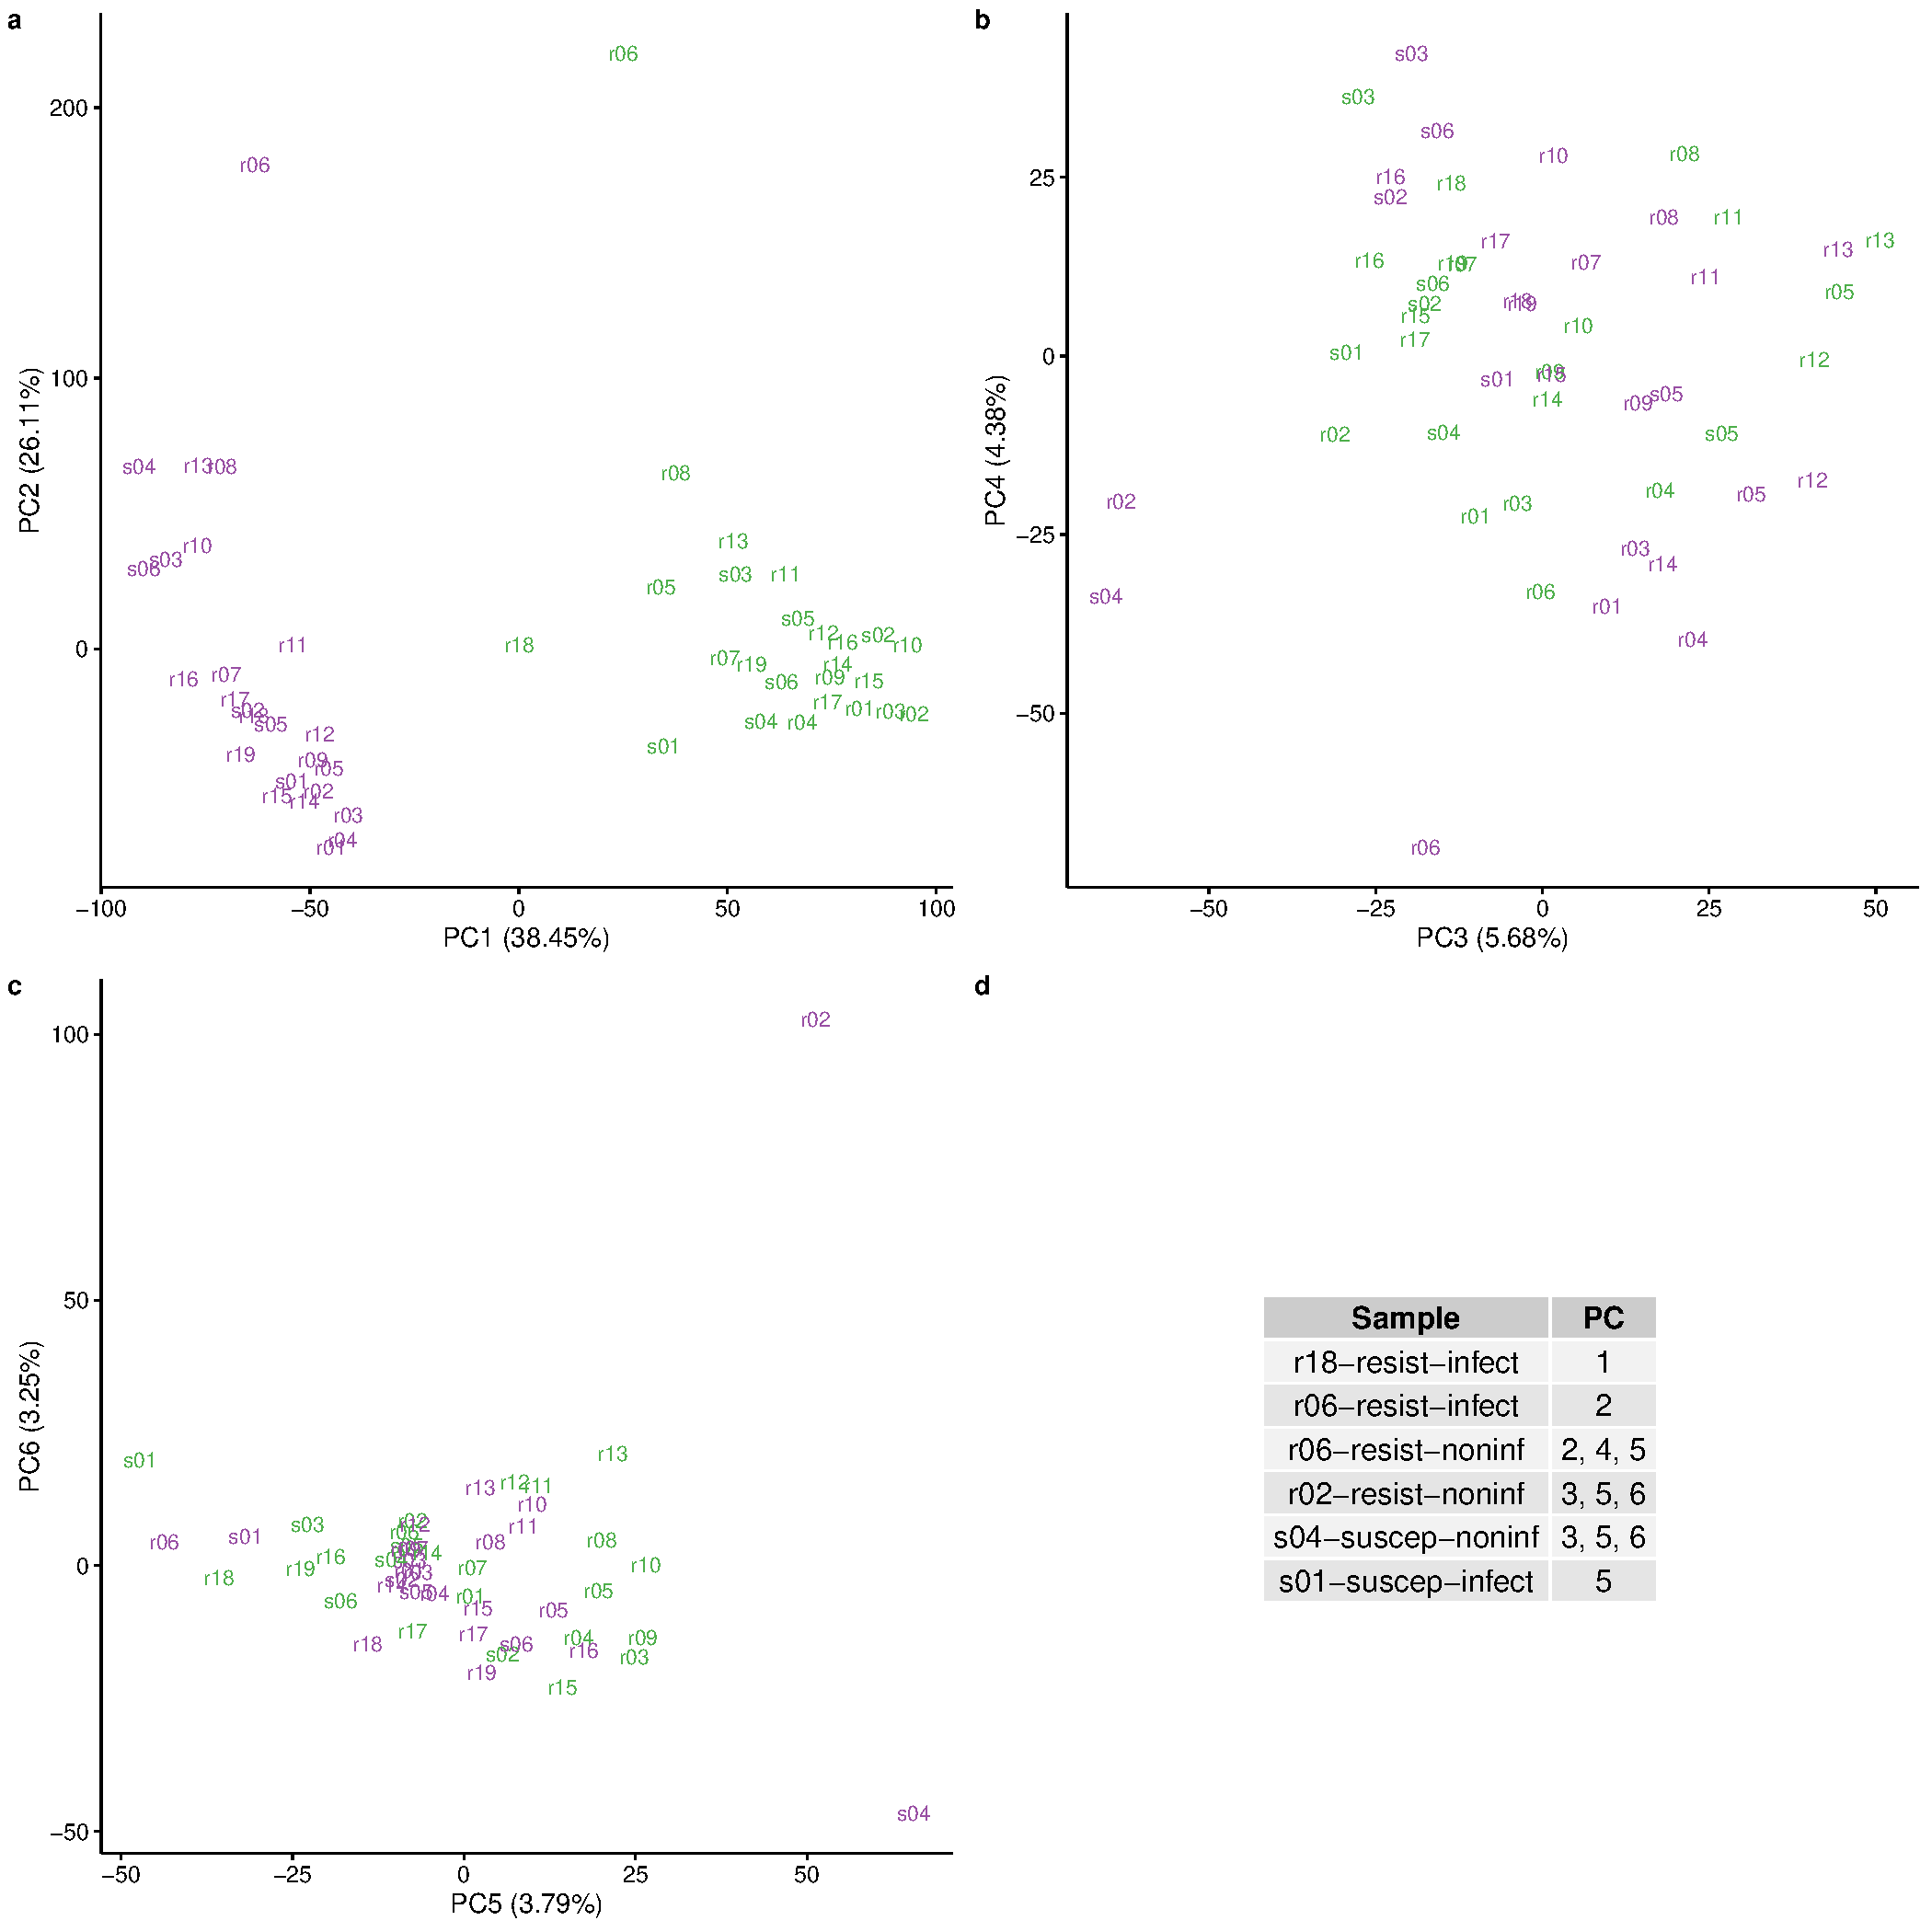
\includegraphics[width=5in]{img/ch03/outliers.pdf}
\caption[Principal components analysis (PCA) to identify outliers.]{
  \textbf{Principal components analysis (PCA) to identify outliers.}
  PC1 versus PC2 (a), PC3 versus PC4 (b), and PC5 versus PC6 (c). Each
  sample is represented by its 3-letter ID. ``s'' stands for
  susceptible and ``r'' for resistant, and the text is colored on the
  basis of treatment status (purple is non-infected; green is
  infected). The value is parentheses in each axis is the percentage
  of total variation accounted for by that PC. The outliers are listed
  in (d). These samples do not fall within 2 standard deviations of
  the mean value of the PCs listed in the right column. Note that a
  separate mean was calculated for the non-infected and infected
  samples for PC1 only.  }
\label{fig:outliers}
\end{figure}


\begin{figure}[!htb]
\centering 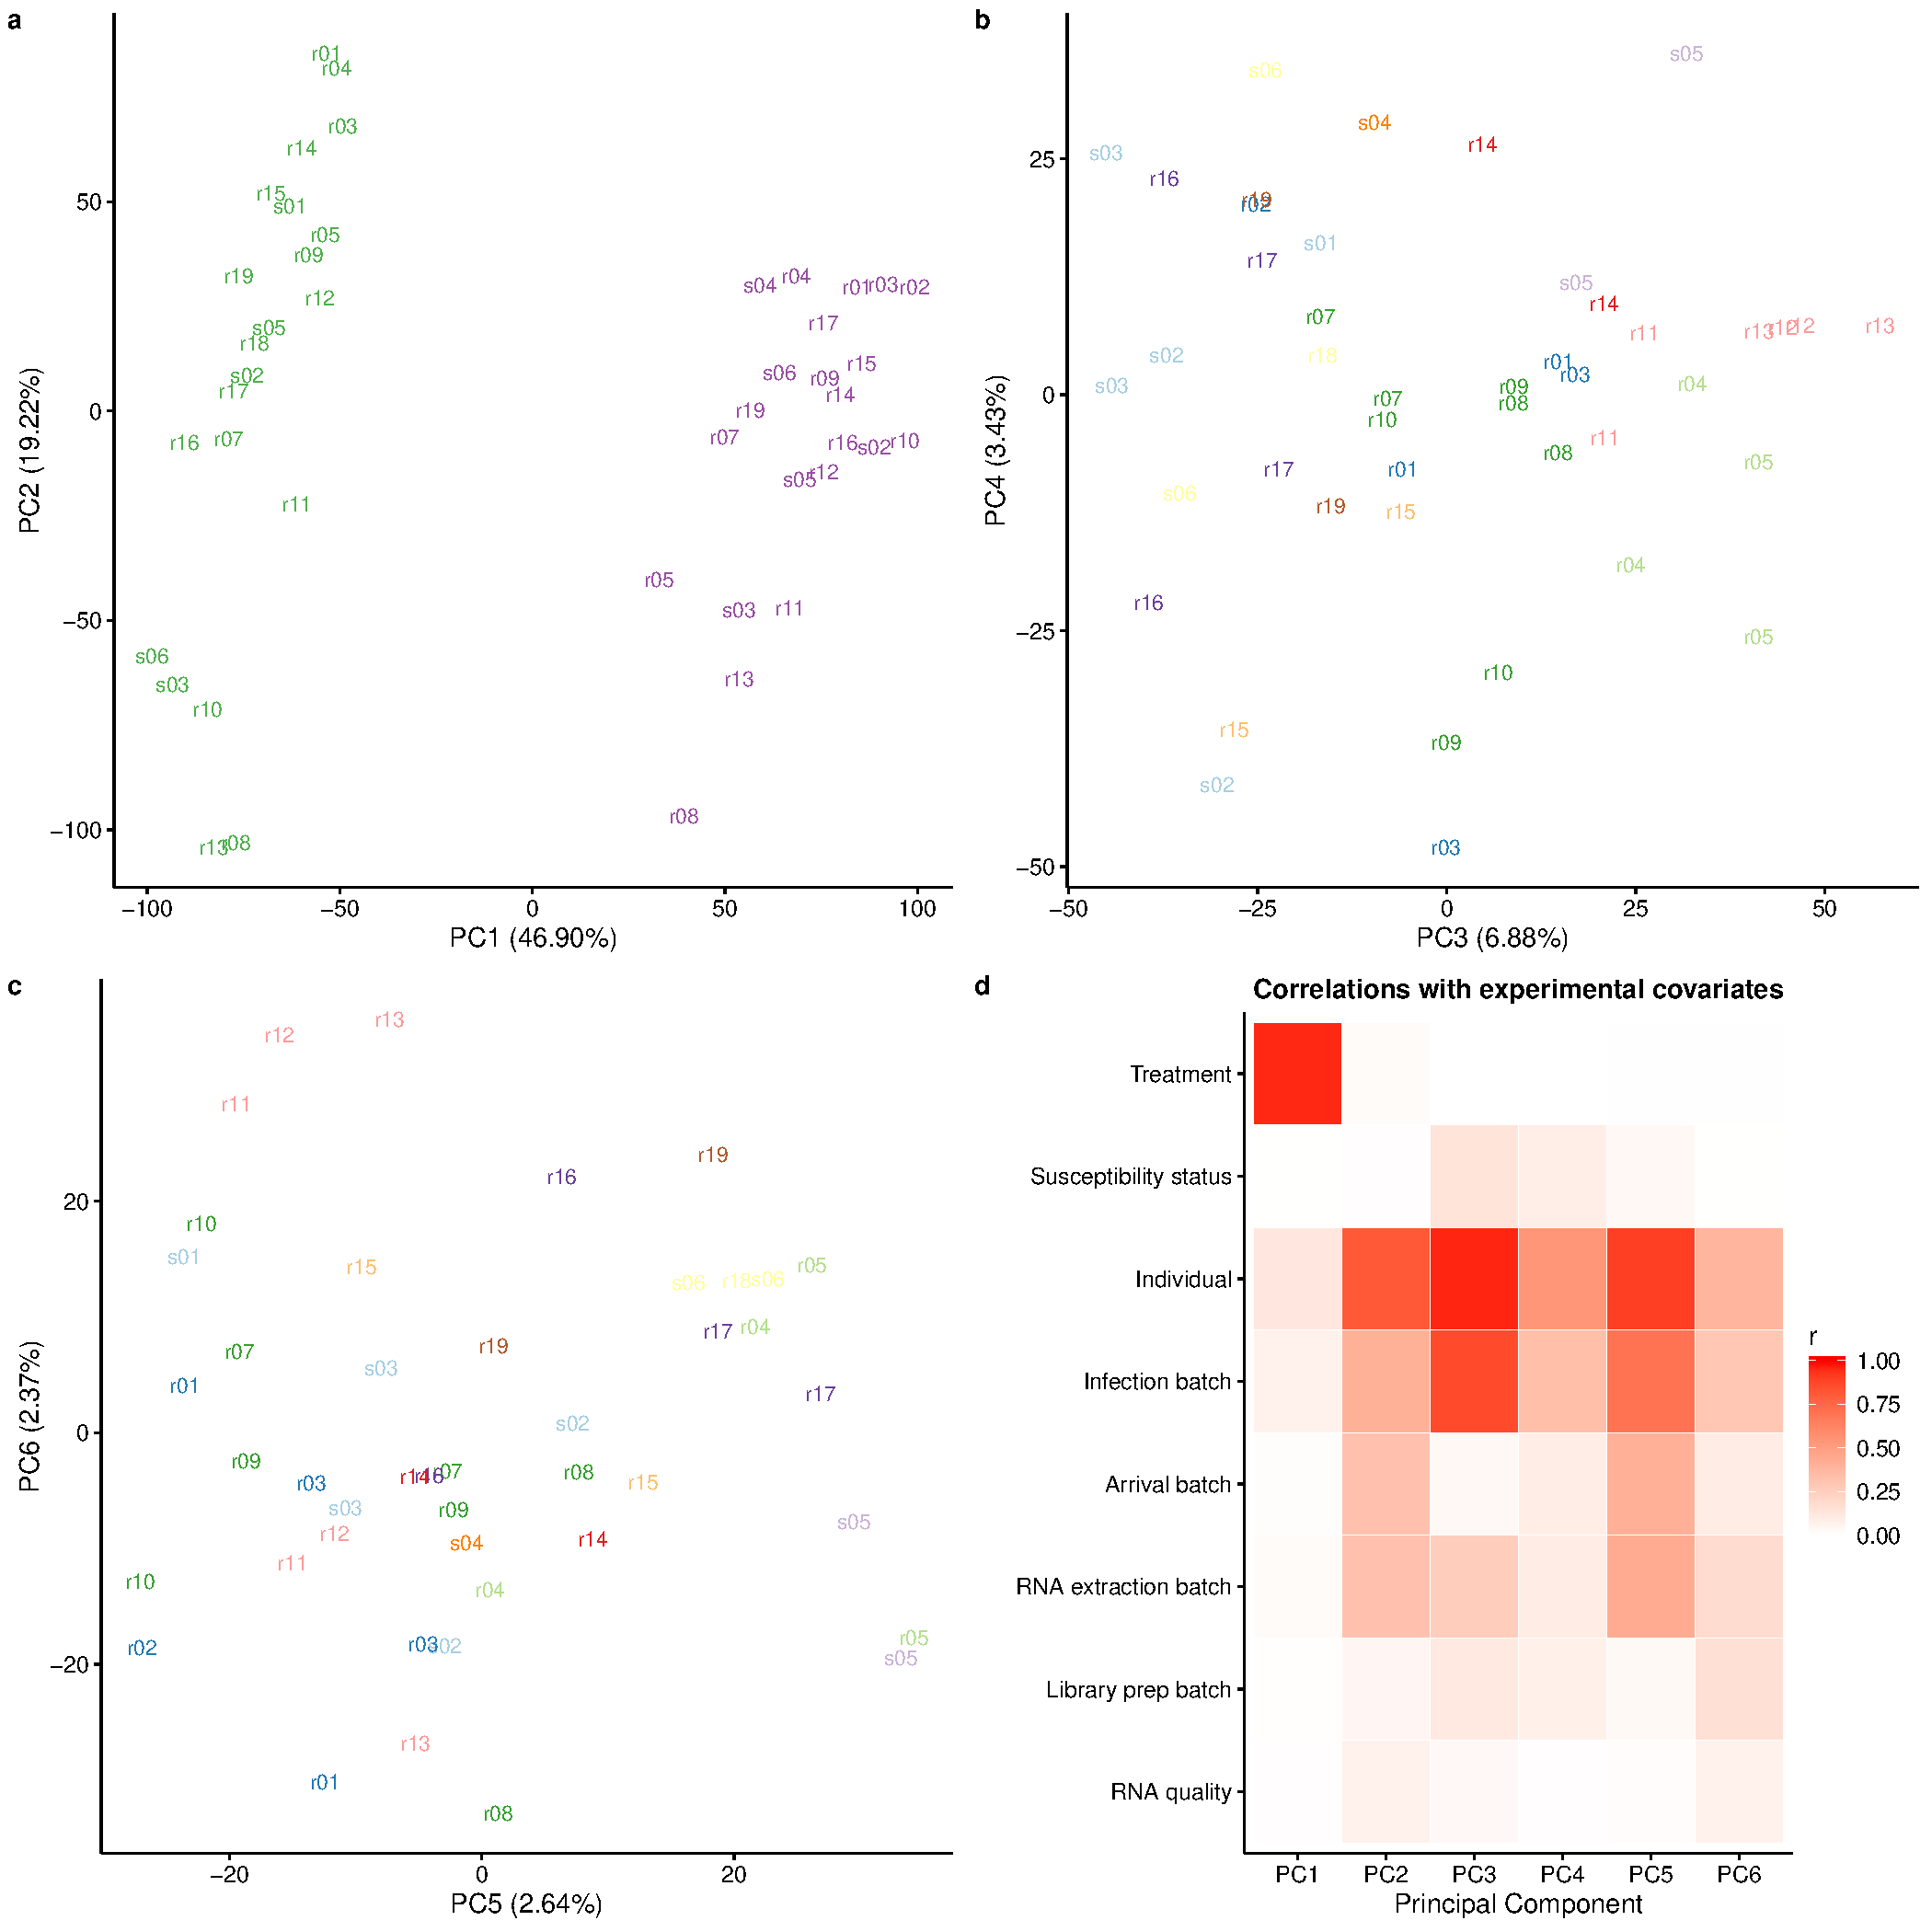
\includegraphics[width=5in]{img/ch03/batch-pca.pdf}
\caption[Check for technical batch effects using principal components
  analysis (PCA).]{ \textbf{Check for technical batch effects using
    principal components analysis (PCA).} (a) PC1 versus PC2. The text
  labels are the individual identifiers. Purple indicates non-infected
  samples and green indicates infected. (b) PC3 versus PC4. The colors
  indicate the different infection batches. (c) PC5 versus PC6. The
  colors indicate the different infection batches. (d) The Pearson
  correlation of PCs 1-6 with each of the recorded biological and
  technical covariates. The correlations vary from 0 (white) to 1
  (red).  }
\label{fig:batch-effect}
\end{figure}

\begin{figure}[!htb]
\centering 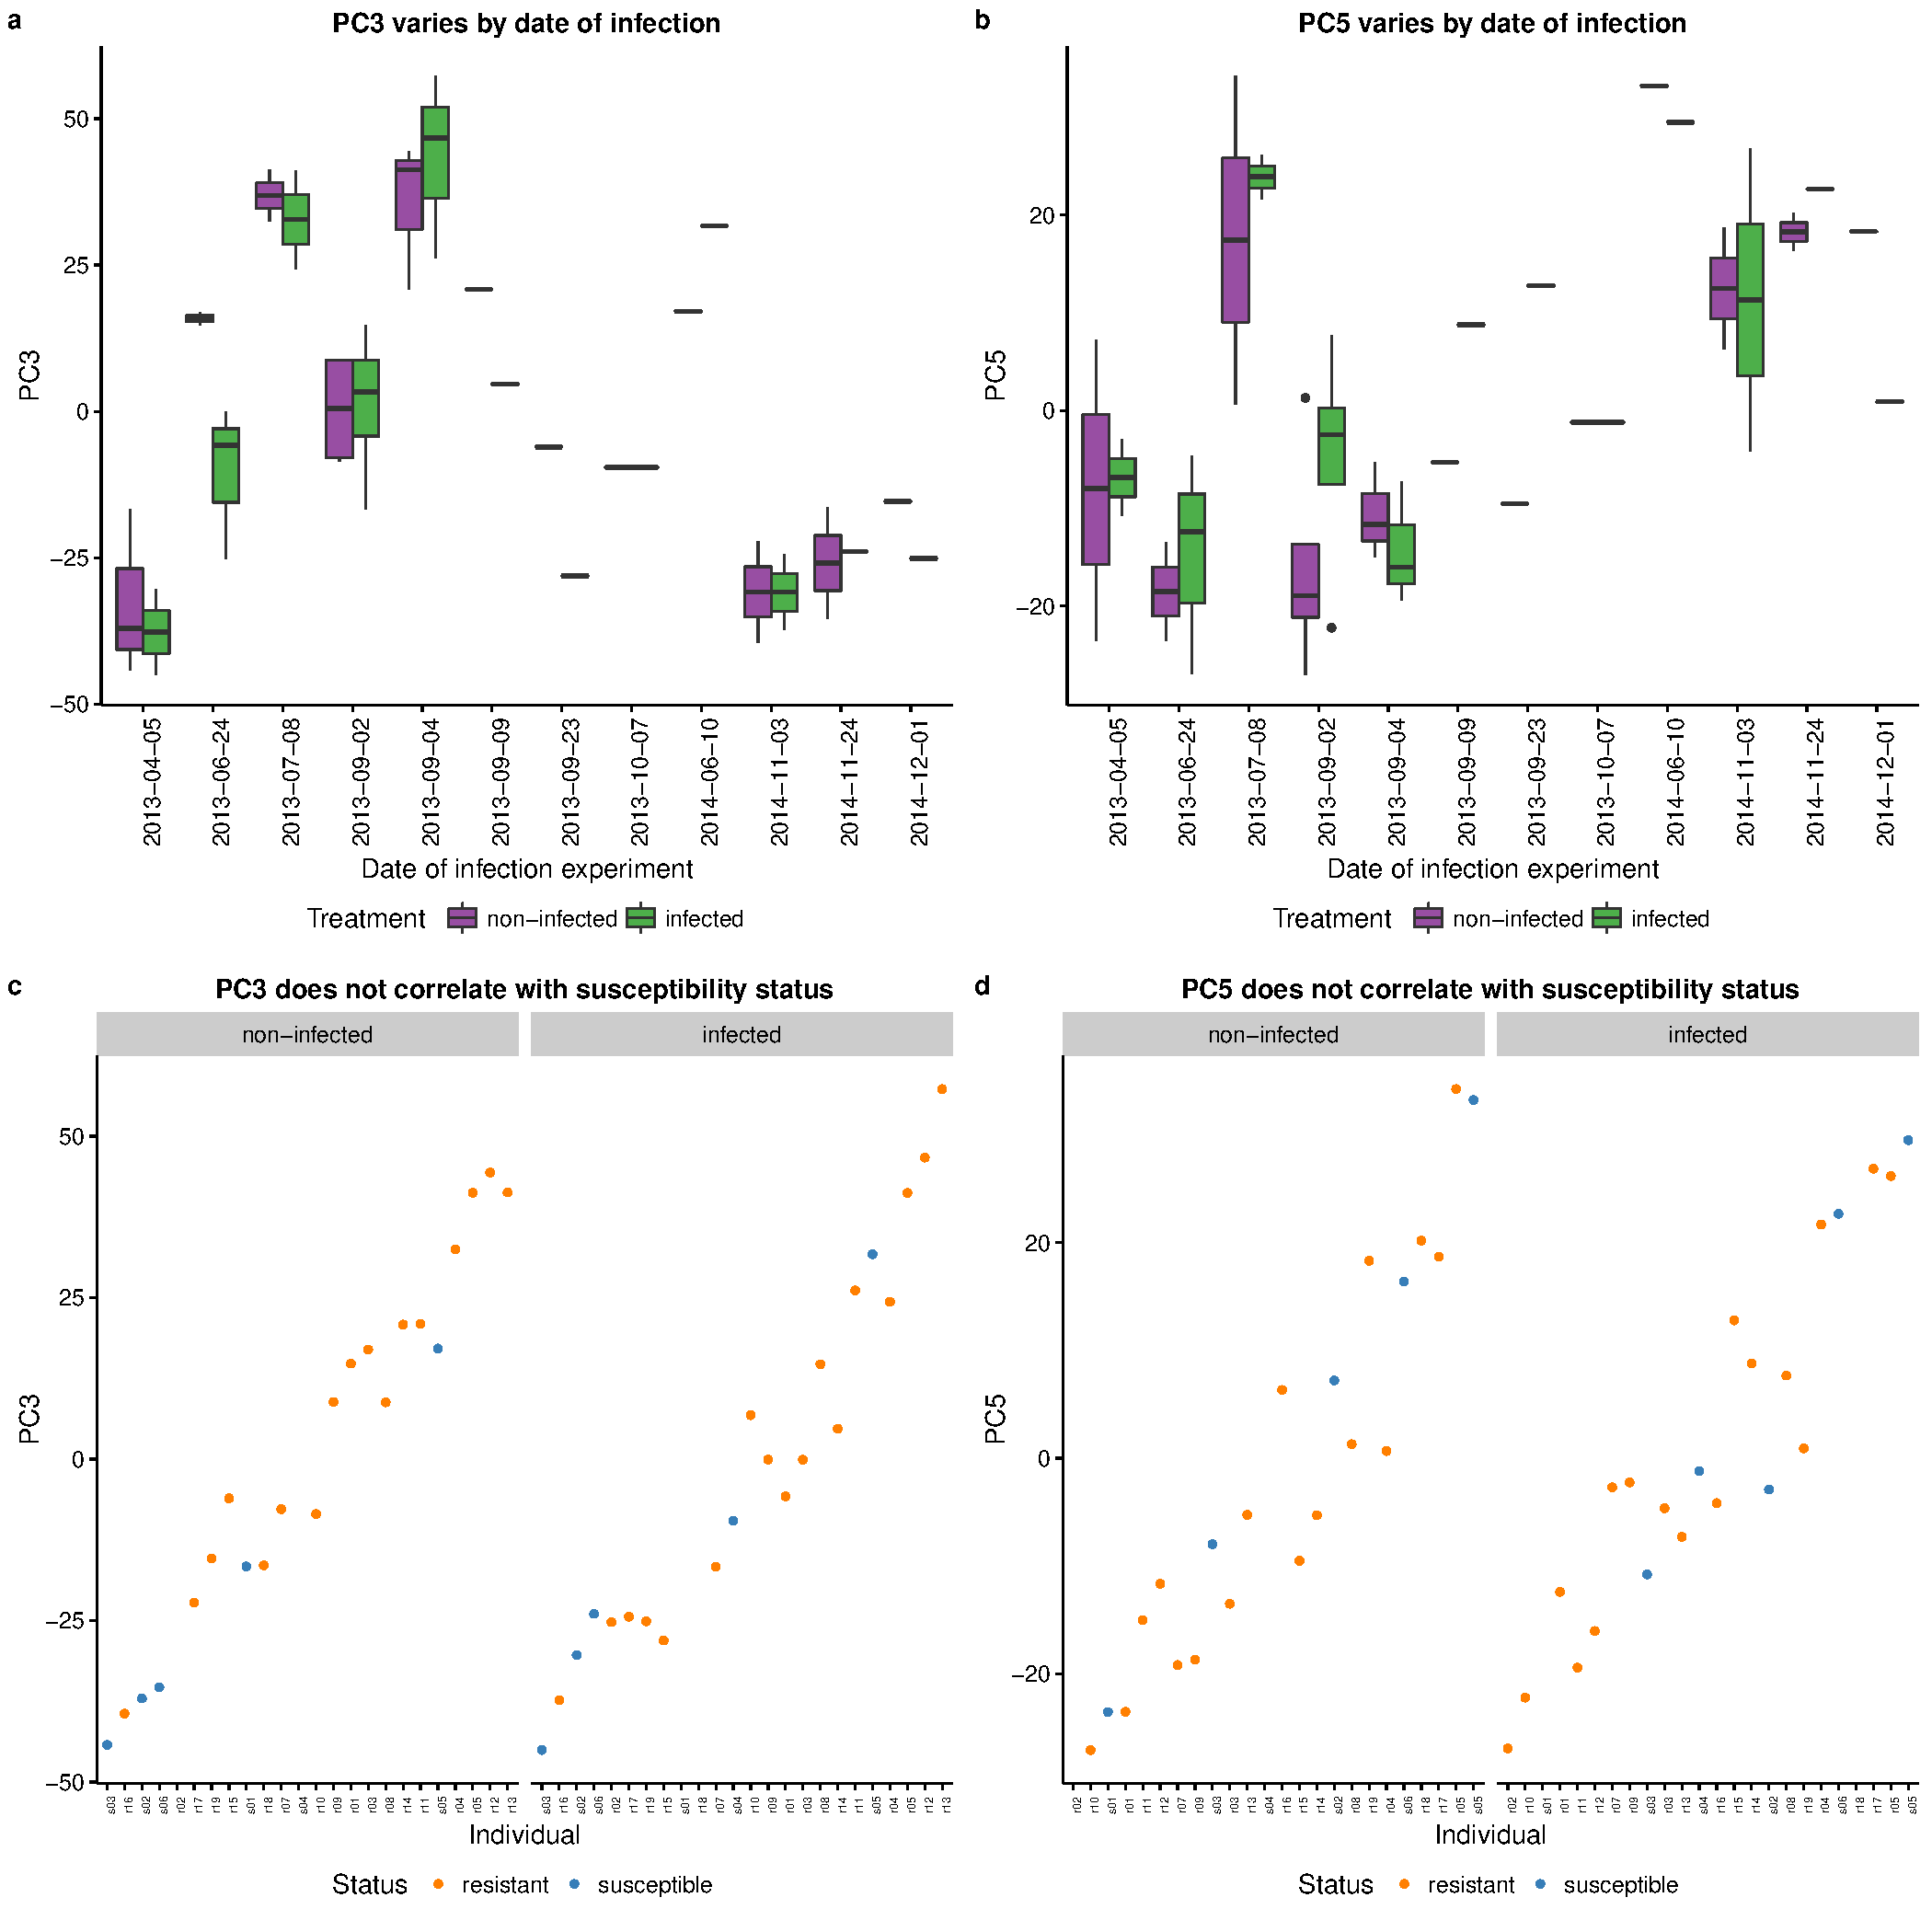
\includegraphics[width=5in]{img/ch03/batch-infection.pdf}
\caption[Check for confounding effect of infection batch.]{
  \textbf{Check for confounding effect of infection batch.} PC3 (a)
  and PC5 (b) varied by the date of infection. Non-infected samples
  are in purple and infected samples in green. Importantly, however,
  this technical variation arising from infection batch did not
  correlate with the susceptibility status of the individuals (c and
  d). Resistant individuals are in orange and susceptible individuals
  in blue.  }
\label{fig:infection}
\end{figure}

\begin{figure}[!htb]
\centering 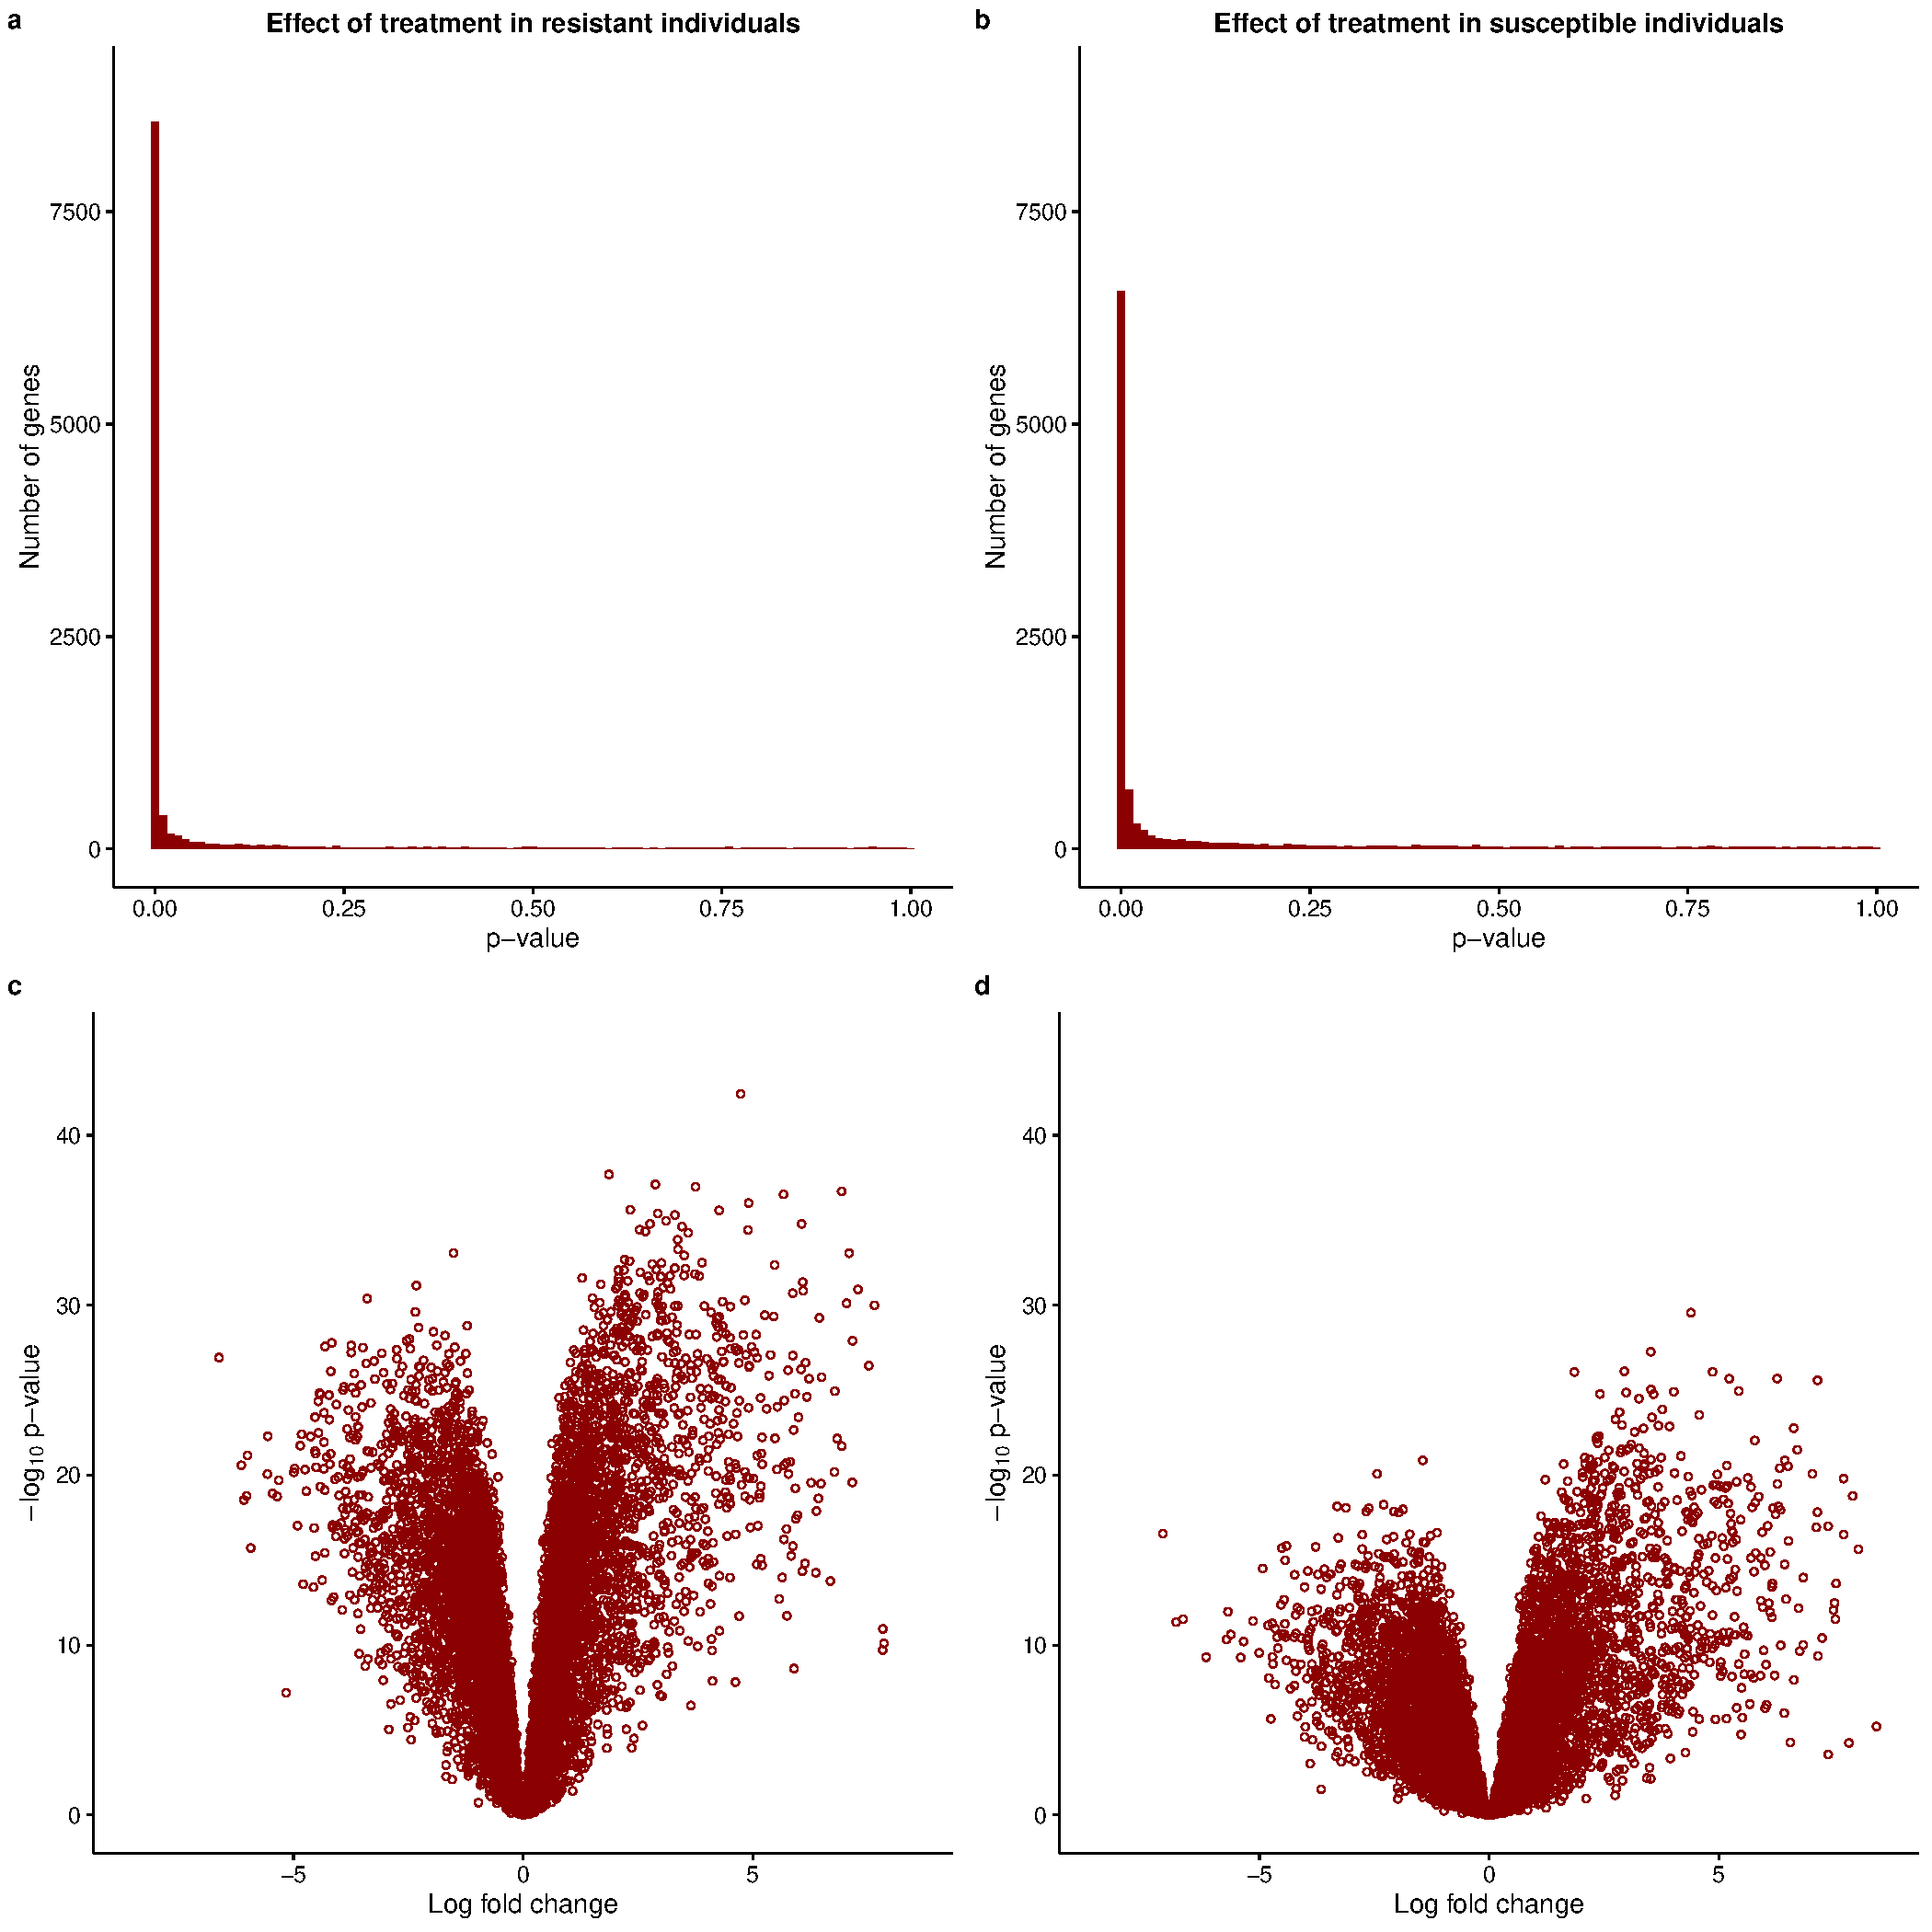
\includegraphics[width=5in]{img/ch03/limma-supp.pdf}
\caption[Effect of treatment with MTB.]{ \textbf{Effect of treatment
    with MTB.} The top panel contains the distribution of unadjusted
  p-values after testing for differential expression between the
  non-infected and infected states in (a) resistant and (b)
  susceptible individuals. The bottom panel contains the corresponding
  volcano plots for the (c) resistant and (d) susceptible individuals.
  The x-axis is the log fold change in gene expression level between
  susceptible and resistant individuals and the y-axis is the
  –log\textsubscript{10} p-value. Red indicates genes which are
  significant differentially expressed with a q-value less than 10\%.
  Because of the extremely skewed p-value distribution, all genes are
  significantly differentially expressed at this false discovery rate.
}
\label{fig:limma-supp}
\end{figure}

\begin{figure}[!htb]
\centering 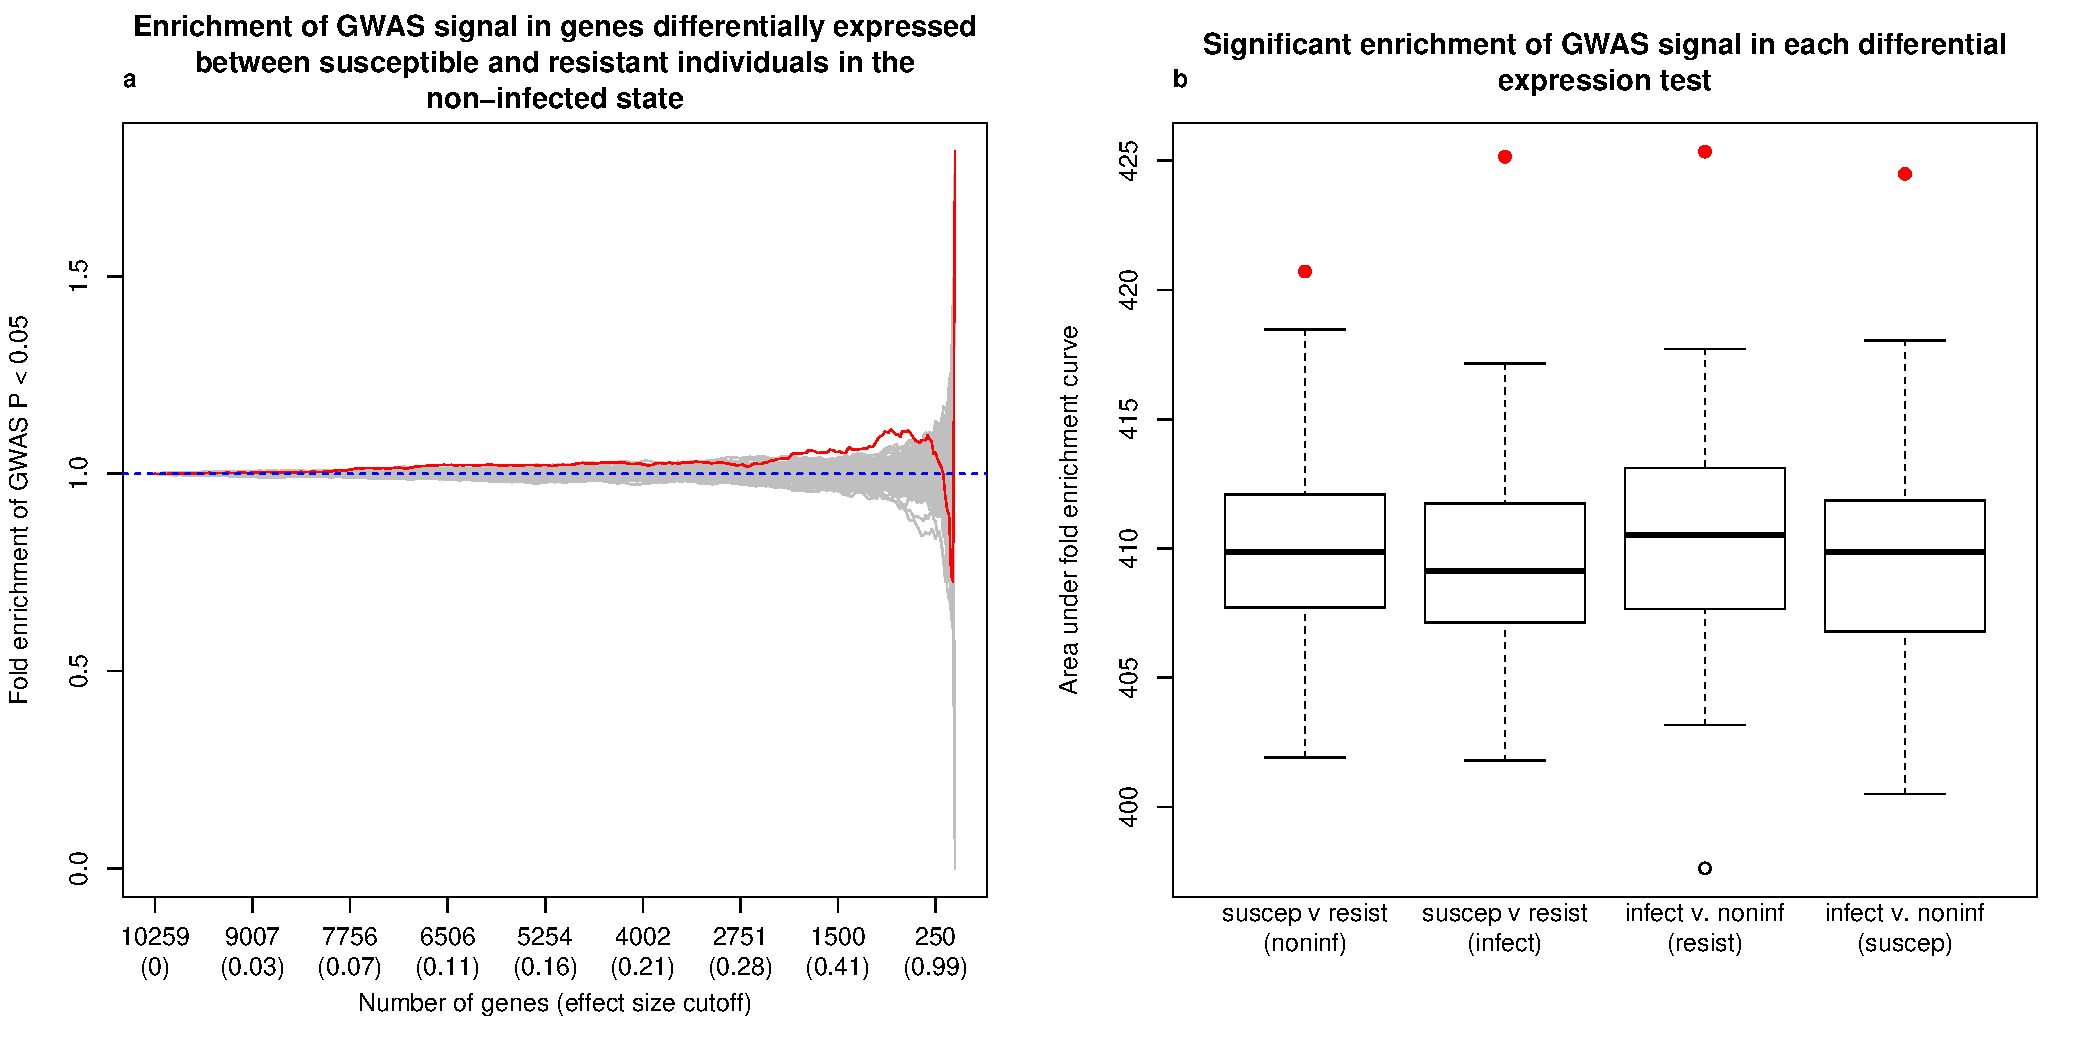
\includegraphics[width=5in]{img/ch03/gwas-supp.pdf}
\caption[Comparison of differential expression and Ghana GWAS
  results.]{ \textbf{Comparison of differential expression and Ghana
    GWAS results.} (a) The y-axis is the fold enrichment (y-axis) of
  genes assigned a SNP with p-value less than 0.05 from the GWAS in
  Ghana \citep{Thye2010}. The x-axis is bins of genes with
  increasingly stringent effect size cutoffs of the absolute log fold
  change between susceptible and resistant individuals in the
  non-infected state. The effect size cutoffs were chosen such that
  each bin from left to right contained approximately 25 fewer
  genes. The red line is the results from the actual data. The grey
  lines are the results from 100 permutations. The dashed blue line at
  y=1 is the null expectation. (b) The x-axis is each of the 4
  differential expression tests performed. The y-axis is the area
  under the curve of the fold enrichment. The boxplot is the result of
  the 100 permutations, and the red point is the result from the
  actual data. As a reference, the leftmost boxplot corresponds to the
  enrichment plot in (a).  }
\label{fig:gwas-supp}
\end{figure}

\begin{figure}[!htb]
\centering
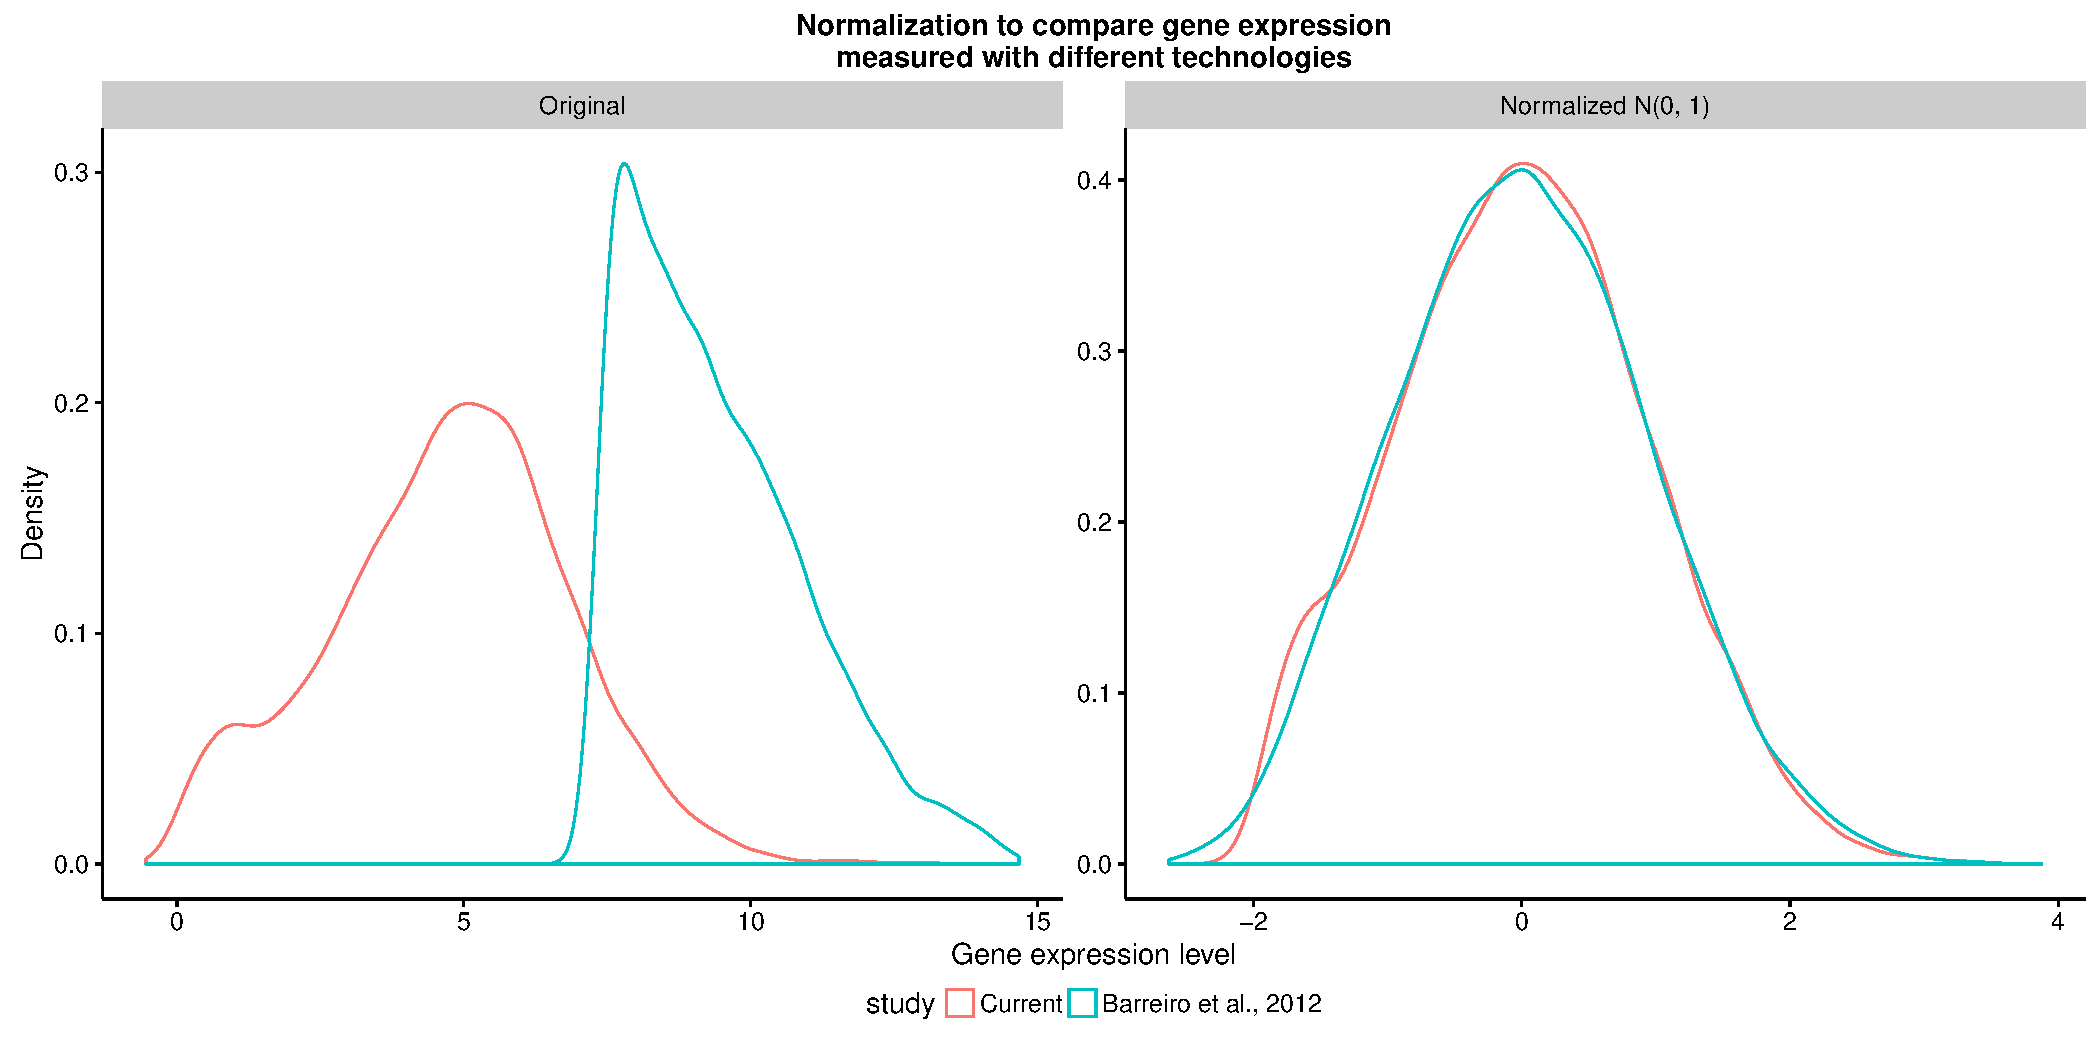
\includegraphics[width=5in]{img/ch03/combined-distributions.pdf}
\caption[Normalizing gene expression distributions.]{
  \textbf{Normalizing gene expression distributions.} (left) The
  distribution of the median log2 cpm of the RNA-seq data from the
  current study in red compared to the distribution of the median gene
  expression levels of the microarray data from Barreiro et al., 2012 in blue. (right) The distributions of the same
  data sets after normalizing each sample to a standard normal
  distribution.  }
\label{fig:combined-dist}
\end{figure}

\begin{figure}[!htb]
\centering 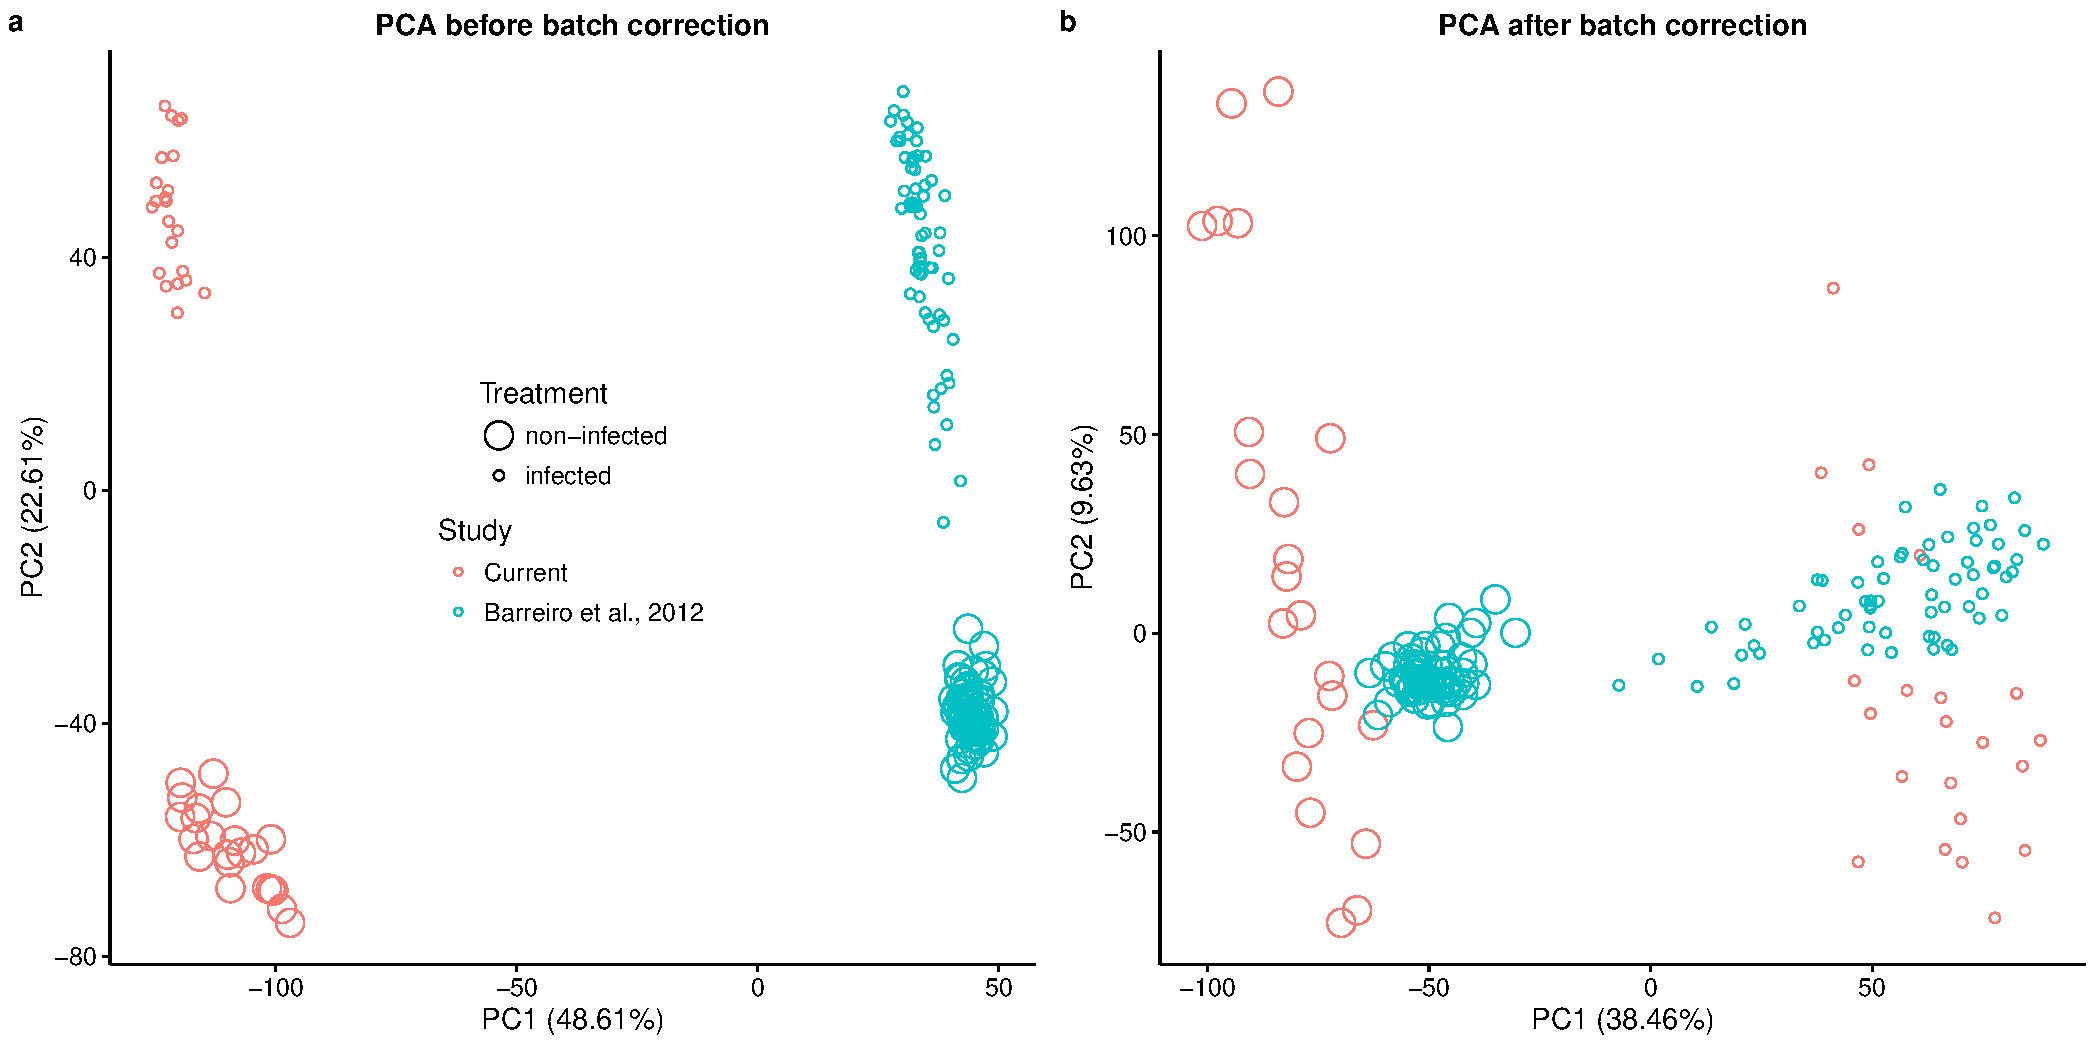
\includegraphics[width=5in]{img/ch03/combined-pca.pdf}
\caption[Principal components analysis (PCA) of combined data sets.]{
  \textbf{Principal components analysis (PCA) of combined data sets.}
  (a) PC1 versus PC2 of the combined data set of the RNA-seq data from
  the current study (red) and the microarray data from Barreiro et
  al., 2012 (blue). The large circles are
  non-infected samples, and the small circles are infected
  samples. The value in parentheses is the percentage of the total
  variation accounted for by that PC. (b) The same data after
  regressing the original PC1 in (a).  }
\label{fig:combined-pca}
\end{figure}

\begin{figure}[!htb]
\centering
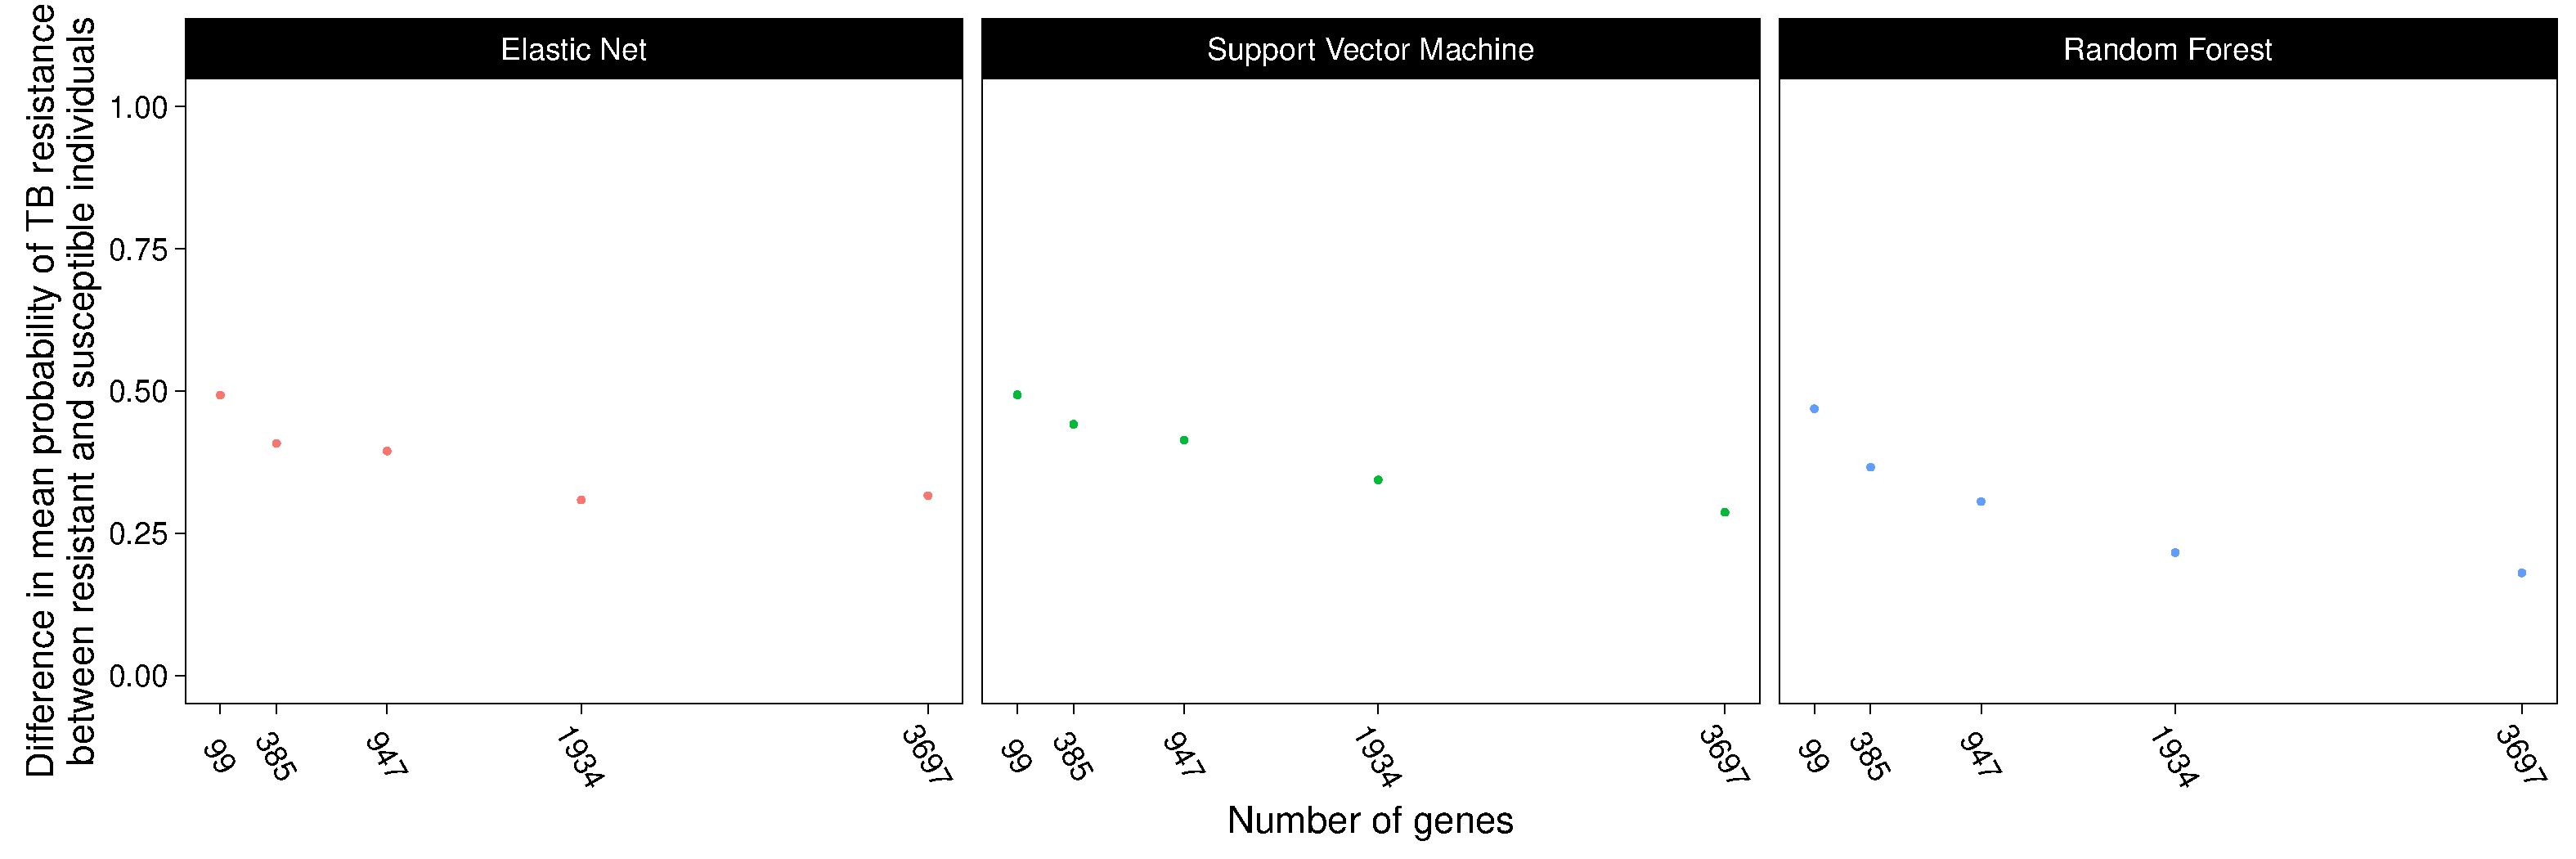
\includegraphics[width=5in]{img/ch03/classifier-compare.pdf}
\caption[Comparing the classification results of different methods and
  number of input genes.]{ \textbf{Comparing the classification
    results of different methods and number of input genes.} We
  compared 3 different machine learning methods (elastic net, support
  vector machine, random forest) and used 5 different sets of input
  genes. The input genes (x-axis) were obtained by varying the q-value
  cutoff for differential expression between susceptible and resistant
  individuals in the non-infected state from 5\% to 25\%. The
  evaluation metric (y-axis) was the difference of the mean assigned
  probability of being TB resistant between the known resistant and
  susceptible individuals in the current study.  }
\label{fig:class-compare}
\end{figure}

\begin{figure}[!htb]
\centering 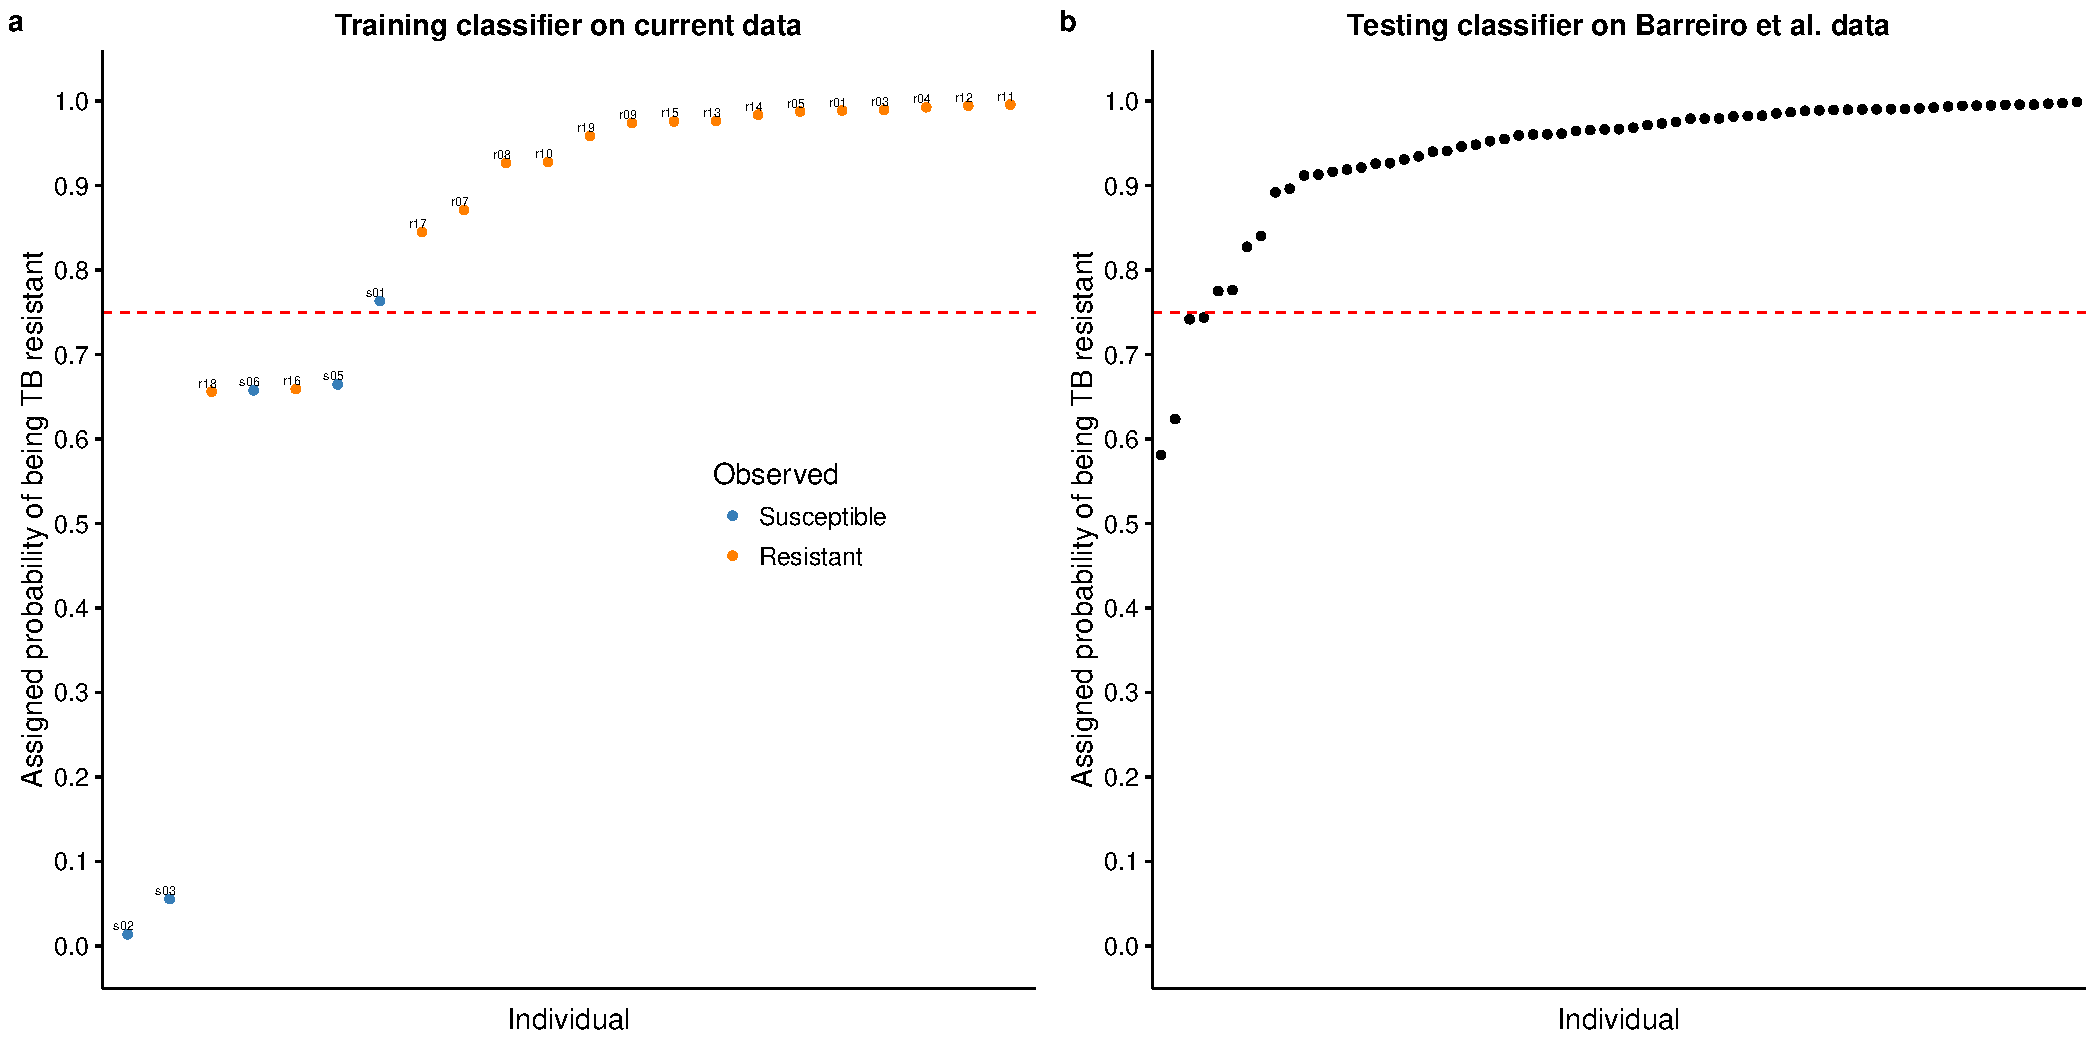
\includegraphics[width=5in]{img/ch03/classifier-en.pdf}
\caption[Classifying TB susceptible individuals using an elastic net
  model.]{ \textbf{Classifying TB susceptible individuals using an
    elastic net model.} (a) The estimates of predicted probability of
  TB resistance from the leave-one-out-cross-validation for
  individuals in the current study.  The blue circles represent
  individuals known to be susceptible to TB, and orange those
  resistant to TB. The horizontal blue line at a probability of 0.75
  almost separates susceptible and resistant individuals. (b) The
  estimates of predicted probability of TB resistance from applying
  the classifier trained on the data from the current study to a test
  set of independently collected healthy individuals  }
\label{fig:class-en}
\end{figure}

\begin{figure}[!htb]
\centering 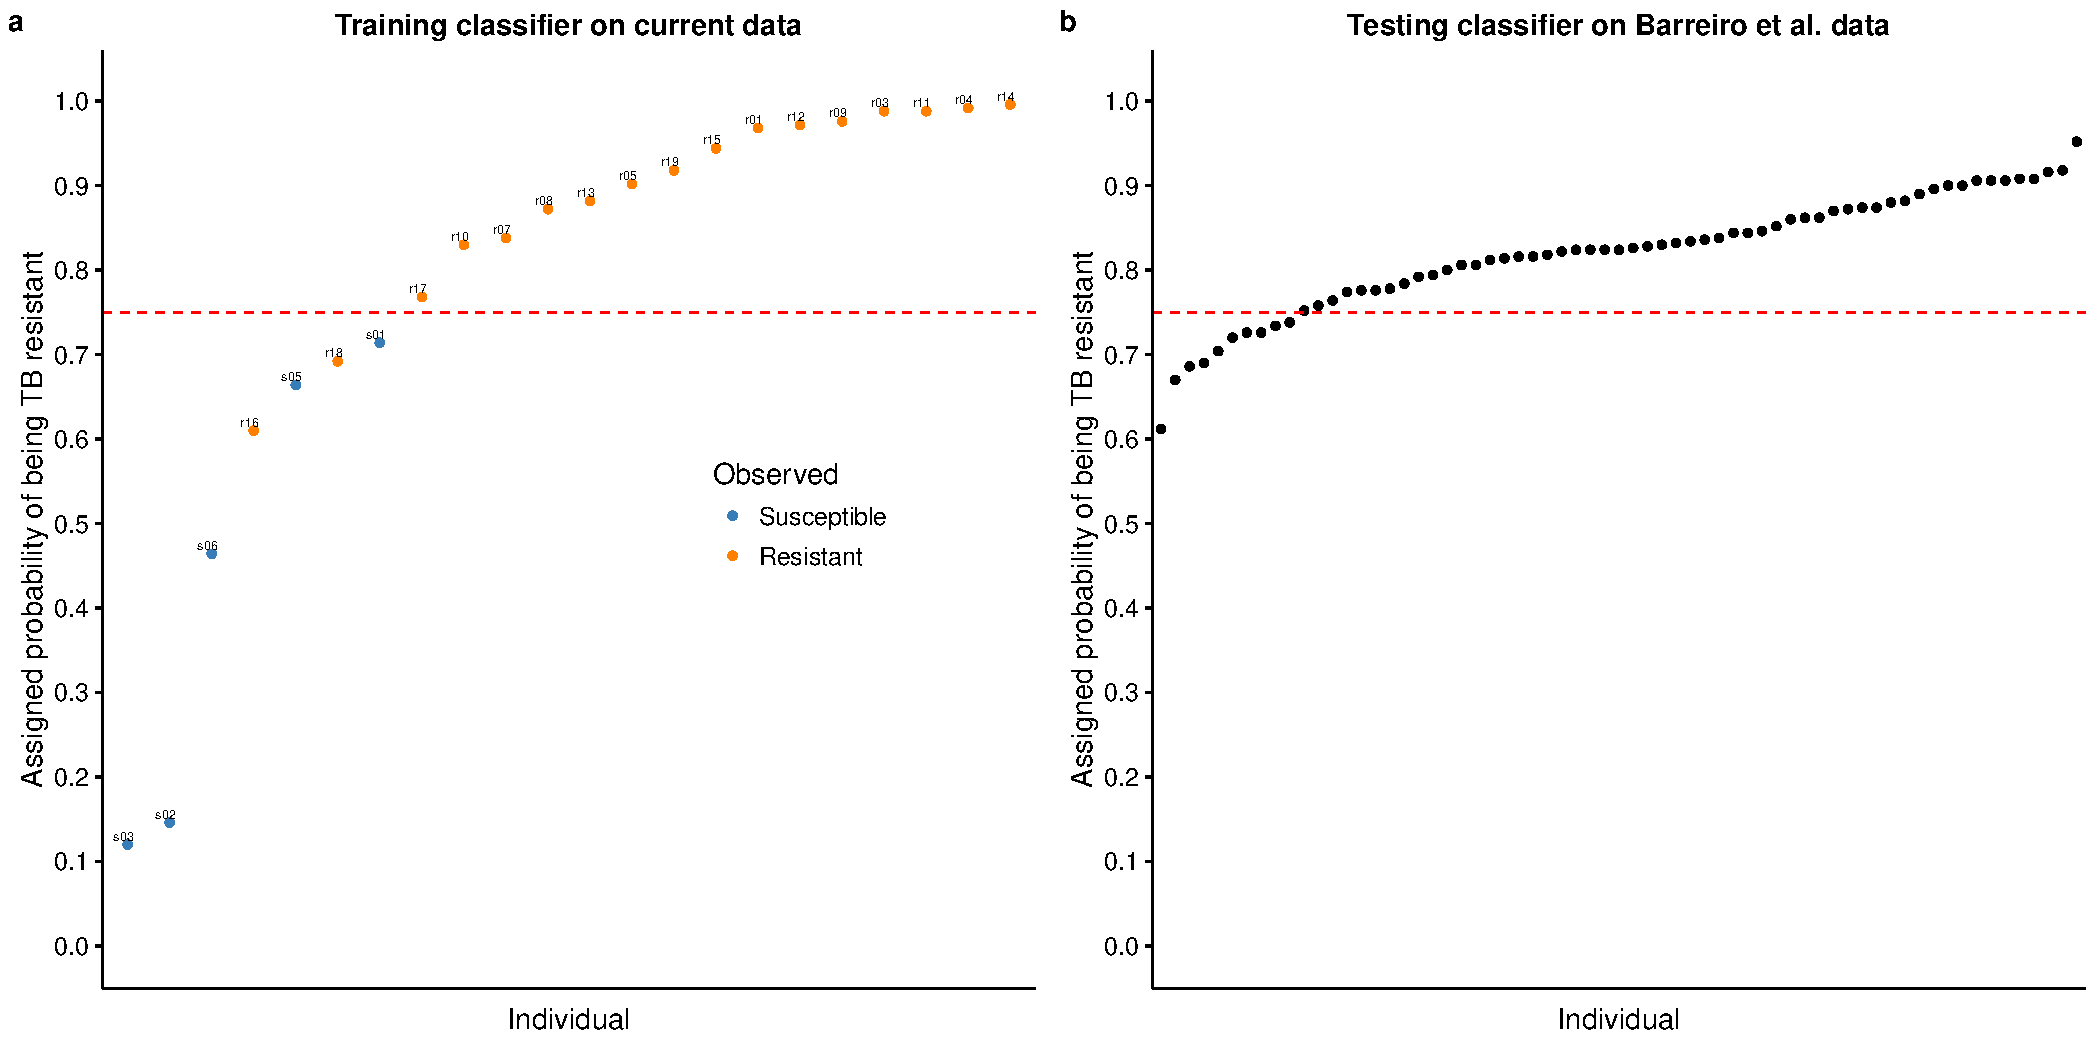
\includegraphics[width=5in]{img/ch03/classifier-rf.pdf}
\caption[Classifying TB susceptible individuals using a random forest
  model.]{ \textbf{Classifying TB susceptible individuals using a
    random forest model.}  (a) The estimates of predicted probability
  of TB resistance from the leave-one-out-cross-validation for
  individuals in the current study.  The blue circles represent
  individuals known to be susceptible to TB, and orange those
  resistant to TB. The horizontal blue line at a probability of 0.75
  separates susceptible and resistant individuals.  (b) The estimates
  of predicted probability of TB resistance from applying the
  classifier trained on the data from the current study to a test set
  of independently collected healthy individuals.
}
\label{fig:class-rf}
\end{figure}

\begin{figure}[!htb]
\centering 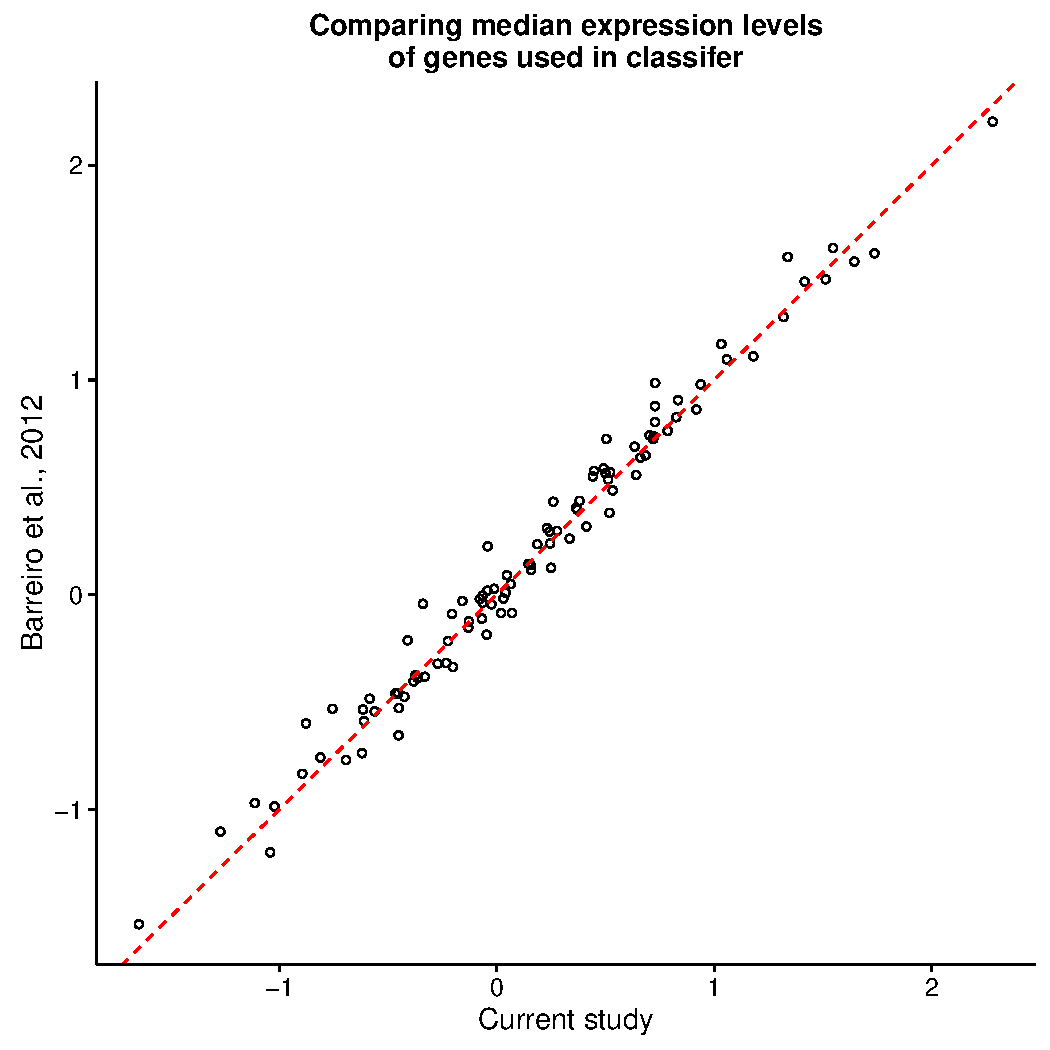
\includegraphics[width=5in]{img/ch03/classifier-exp.pdf}
\caption[Comparing gene expression between the two studies.]{
  \textbf{Comparing gene expression between the two studies.} After
  normalization and batch-correction, the median expression levels of
  the 99 genes used in the classifier were similar between the samples
  in the current study and those in Barreiro et al., 2012. The dashed red line is the 1:1 line.  }
\label{fig:class-exp}
\end{figure}

